In this section, we explain the meaning of the problems in \texttt{SIPLIB 2.0}. For each problem, we provide the extensive form formulation which we believe the clearest way to describe what the problem wants to do. We also give numerical parameter values together with random data generation procedures. Due to the limited access to the original data in reference papers, we sometimes selectively choose the methods from several available references and modify them without harming validity. Also, we guess some parameters about scenario generation to connect the missing links. The information in this section is completely implemented and contained in the accompanied \julia\ package: \texttt{Siplib/src/problems}. We recommend users to take a look inside the \julia\ implementation to verify the conformance of all the details.

\subsection{\airlift: Airlift operations scheduling} \label{AIRLIFT}
\airlift\ is a scheduling problem that allocates flight routes and flying number for different types of aircraft to meet uncertain cargo demands from all routes. Each aircraft type has limited number of available flying hours and different flight hours/costs. In the first stage, the number of flights and corresponding routes are initially assigned to each aircraft type. The second stage recourse action includes reallocation of flight time/route and purchase of commercial transportation. Switching aircraft from one route to another causes increased hours/costs than it is supposed to be. Moreover, it sometimes gives rise to cancellation of initially assigned flights due to the different flying ability for each type.    

Fig. \ref{fig:airlift_sparsity} shows the sparsity pattern presents in extensive form \airlift\ (single scenario).
\begin{figure}[H]
	\centering
	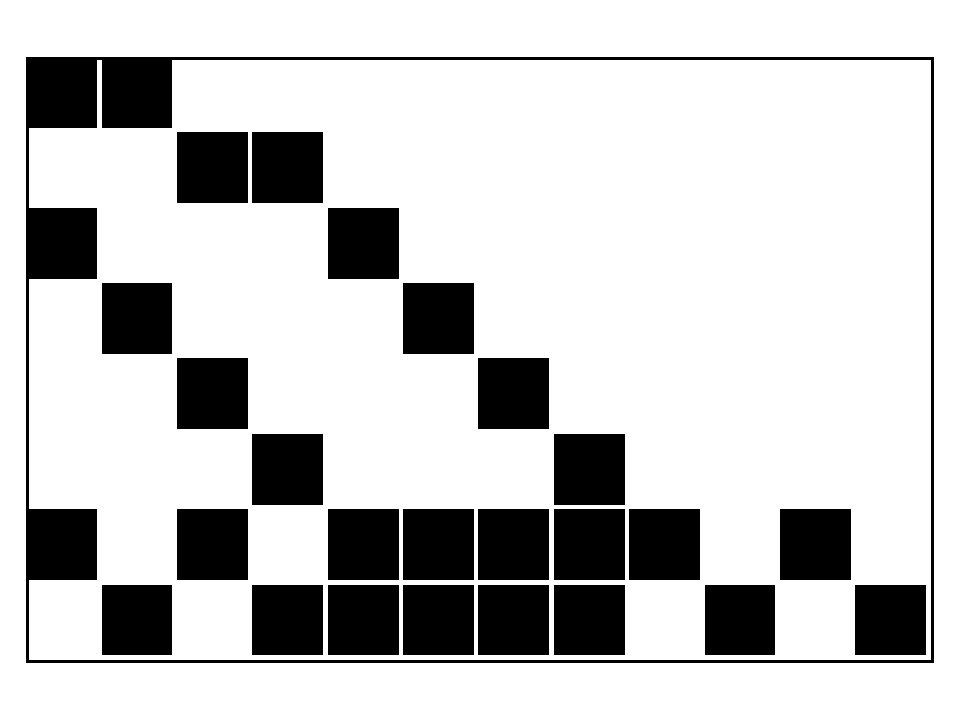
\includegraphics[width=0.85\linewidth]{AIRLIFT_1}
	\caption{AIRLIFT\_1: Extensive form constraint matrix plot}
	\label{fig:airlift_sparsity}
\end{figure}
\subsubsection{\airlift: Mathematical formulation}
Table \ref{airlift:notation} summarizes the notation used to formulate \airlift. Using the notation, the problem can be formulated by the following extensive form.
\begin{subequations} \label{airlift:formulation}
	\begin{align}
	(\airlift)\ \textrm{min}\ &\sum_{i\in A}\sum_{j\in R} c_{ij}x_{ij}+\sum_{s\in\mathcal{S}}\PP(s)\Bigg[ \sum_{i\in A}\sum_{j\in R}\sum_{k\in R\backslash \{j\} }\left( \gamma_{ijk}-c_{ij}\frac{\alpha_{ijk}}{a_{ij}} \right)\chi_{ijk}^s \nonumber \\ 
	&\qquad\qquad\qquad\qquad\qquad\qquad\qquad\qquad+\sum_{j\in R}\left( c_j^+ y_j^{+s}+c_j^- y_j^{-s} \right)\Bigg]\label{airlift:obj} \\
	\textrm{s.t.}\ & \sum_{j\in R}a_{ij}x_{ij}\le F_i,\quad\forall i\in A,	\label{airlift:b}\\
	&\sum_{k\in R\backslash\{j\}}\alpha_{ijk}\chi_{ijk}^s\le a_{ij}x_{ij},\quad\forall i\in A,\ \forall j\in R,\ \forall s\in\mathcal{S}, \label{airlift:c}\\
	&\sum_{i\in A}b_{ij}x_{ij}-\sum_{i\in A}\sum_{k\in R\backslash\{j\}}b_{ij}\left(\frac{\alpha_{ijk}}{a_{ij}}\right)\chi_{ijk}^s + \sum_{i\in A}\sum_{k\in R\backslash\{j\}}b_{ij}\chi_{ikj}^s \nonumber \\
	&\qquad\qquad\qquad\qquad\qquad\quad+ y_j^{+s} - y_j^{-s} = d_j^s,\quad \forall j\in R,\ \forall s\in\mathcal{S}, \label{airlift:d}\\
	&x_{ij}\in\mathbb{Z}_+,\quad\forall i\in A,\ \forall j\in R, \label{airlift:e}\\
	&\chi_{ijk}^s\in\mathbb{Z}_+,\quad\forall i\in A,\ \forall j\in R,\ \forall k\in R\backslash\{j\},\ \forall s\in\mathcal{S}, \label{airlift:f}\\
	& y_j^{+s},y_j^{-s}\ge 0,\quad\forall j\in R,\ \forall s\in\mathcal{S}.\label{airlift:g}
	\end{align}
\end{subequations}
The objective function (\ref{airlift:obj}) minimizes the total operating costs including penalty costs. Constraint (\ref{airlift:b}) restricts the maximum number of flight hours for each aircraft type available during the month. Constraint (\ref{airlift:c}) corresponds the fact that we cannot switch away more flight hours. Constraint (\ref{airlift:d}) balances the demand and supply for each route considering the unused capacity together. Constraint (\ref{airlift:e})-(\ref{airlift:g}) set the space in which the decision variables can have values.

\begin{table}[H]
	\caption{Notations for \airlift}
	\label{airlift:notation}
	\resizebox{\textwidth}{!}
	{
%		{@{}llp{3in}}
		\begin{tabular}{ll}
			\toprule
			\multicolumn{2}{l}{\textbf{Index sets:}} \\
			$A$ & index set of aircraft types ($i,k\in A$)\\ 
			$R$ & index set of flying routes ($j\in R$)\\ 
			$\mathcal{S}$ & index set of scenarios ($s\in \mathcal{S}$) \\ \midrule
			\multicolumn{2}{l}{\textbf{Parameters:}} \\
			$F_i$ & the maximum number of flying hours for aircraft of type $i$ available during the month\\
			$a_{ij}$ & number of hours that aircraft type $i$ requires to fly an initially assigned route $j$  \\
			$\alpha_{ijk}$ & number of hours that a re-scheduled aircraft of type $i$ requires to fly route $k$ where the initially assigned route was $j$ ($\alpha_{ijk}\ge a_{ik}$)\\
			$b_{ij}$ & carrying capacity of a flight of an aircraft type $i$ on route $j$\\
			$c_{ij}$ & cost per flight of aircraft type $i$ initially assigned to and flown on route $j$ ($c_{ij}\ge 0$)\\
			%$\gamma_{ijk} $& cost per flight of aircraft type $i$ assigned to route $k$ that uses hours made available by canceling flights on route $j$ ($\gamma_{ijk}\ge c_{ik}$)\\			
			$\gamma_{ijk} $& cost per flight of aircraft of type $i$ whose flying route is re-assigned from $j$ to $k$ ($\gamma_{ijk}\ge c_{ik}$)\\			
			$c_j^+$ & unit cost of meeting demand by commercial transport on route $j$\\
			$c_j^-$ & unit penalty cost of unused capacity on route $j$\\
			$d_j^s$ & total demand for route $j$ under scenario $s$ \\
			$\PP(s)$ & \textrm{the probability of occurence of scenario $s$} \\ \midrule
			\multicolumn{2}{l}{\textbf{Decision variables:}} \\
			$x_{ij}$ (1st-stage) & number of flights of aircraft type $i$ initially assigned to route $j$ \\
			$\chi_{ijk}^s$ (2nd-stage) & number re-scheduled flights of aircraft type $i$ from route $j$ to $k$ \\ 
			$y_j^{+s}$ (2nd-stage) & amount of demand carried by commercial transportation on route $j$ under scenario $s$\\
			$y_j^{-s}$ (2nd-stage) & amount of unused capacity on route $j$ under scenario $s$\\
			\bottomrule
		\end{tabular}
	}
\end{table} 

\subsubsection{\airlift: Data generation}
The original reference \cite{journal:MW1969} provides a numerical example with $|A|=2$ and $|R|=2$ (Table \ref{AIRLIFT:numeric}). 

\begin{table}[H]
	\caption{\airlift: Numerical data in \cite{journal:MW1969}}
	\label{AIRLIFT:numeric}
	\centering
	\resizebox{\textwidth}{!}{%
		\begin{tabular}{cccccccccccc}
			\hline
			\multirow{2}{*}{\begin{tabular}[c]{@{}c@{}}Aircraft \\ type $(i)$\end{tabular}} & \multicolumn{2}{c}{$a_{ij}$ (hours)} & \multicolumn{2}{c}{$b_{ij}$ (tons)} & \multicolumn{2}{c}{$c_{ij}$ (dollars)} & $\alpha_{ijk}-a_{ij}$ (hours) & $\gamma_{ijk}-c_{ij}$ (dollars) & \multicolumn{2}{c}{$c_j^+$ (dollars)}       & $c_j^-$ (dollars)\$ \\ \cline{2-12} 
			& $j=1$             & $j=2$            & $j=1$            & $j=2$            & $j=1$              & $j=2$             & $\forall (j,k)$               & $\forall (j,k)$                 & $j=1$                & $j=2$                & $j=1,2$             \\ \hline
			1                                                                               & 24                & 14               & 50               & 75               & 7200               & 6000              & 5                             & 1000                            & \multirow{2}{*}{500} & \multirow{2}{*}{250} & \multirow{2}{*}{0}  \\
			2                                                                               & 49                & 29               & 20               & 20               & 7200               & 4000              & 7                             & 1500                            &                      &                      &                     \\ \hline
		\end{tabular}%
	}
\end{table}
According to the original reference, demand on each route is lognormally distributed with mean and standard deviation pairs (1000, 50) and (1500, 300). To get the desired result, we generate random numbers from the following lognormal distributions:
\begin{align*}
d_1^s&=Lognormal(\mu=6.906,\ \sigma=0.05),\quad\forall s\in\mathcal{S},\\
d_2^s&=Lognormal(\mu=7.2936,\ \sigma=0.198),\quad\forall s\in\mathcal{S}.
\end{align*}


\subsection{\cargo: Cargo network scheduling} \label{CARGO}
\cargo\ is a two-stage cargo network scheduling problem. The problem is to plan flights over the possible routes in a network in order to ship cargo from some nodes to other nodes. The cargo amounts to be shipped between two nodes are uncertain. The first-stage decision is to determine the number of flights on each route by a certain type of aircraft. We allow cargo to be moved either by direct delivery by a single route, or by transshipment, i.e., by more than one route. Then, the second-stage decision must satisfy the maximum capacity constraints towards minimizing total costs by considering both direct delivery and transshipment.

Fig. \ref{fig:cargo_sparsity} shows the sparsity pattern presents in extensive form \cargo\ (single scenario).
\begin{figure}[H]
	\centering
	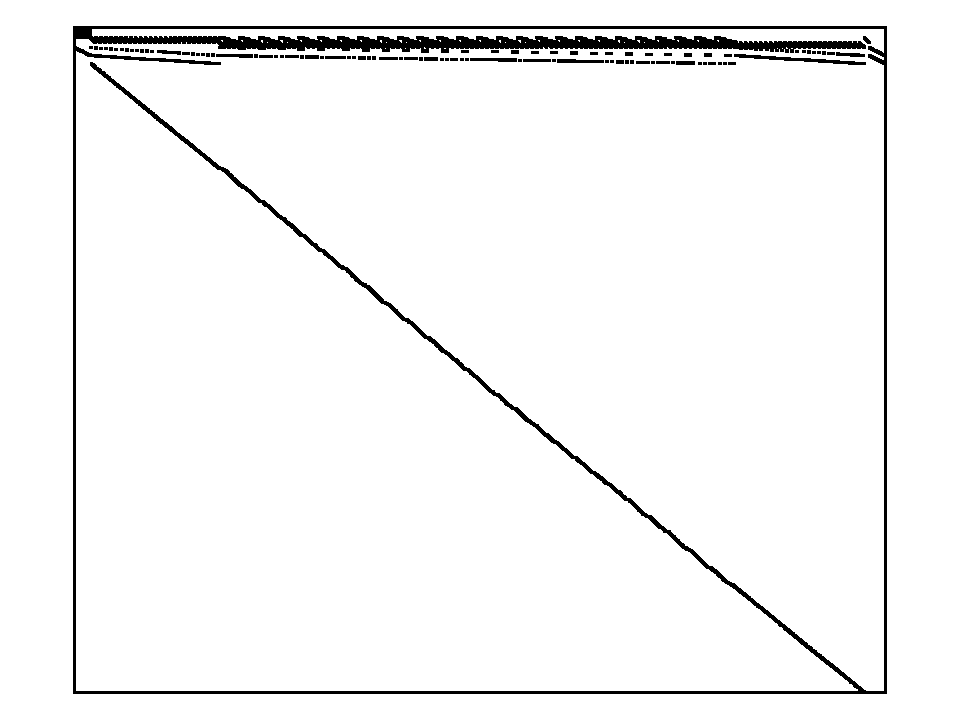
\includegraphics[width=0.85\linewidth]{CARGO_1}
	\caption{CARGO\_1: Extensive form constraint matrix plot}
	\label{fig:cargo_sparsity}
\end{figure}
\subsubsection{\cargo: Mathematical formulation}
Table \ref{cargo:notation} summarizes the notation used to formulate \cargo. Using the notation, the problem can be formulated by the following extensive form.
\begin{subequations} \label{cargo:formulation}
	\begin{align}
	(\cargo)\ \textrm{min}\ &\sum_{\pi\in P}\sum_{a\in A}c_a h_{\pi a}x_{\pi a}+ \nonumber \\ &\sum_{s\in\mathcal{S}}\PP(s)\left[q\sum_{\pi\in P}\sum_{(m,n)\in\pi}\left(d_{\pi m n}^s+r_{\pi m n}^s+\sum_{k\in N}t_{\pi m n k}^s\right)+\rho\sum_{m\in N}\sum_{n\in N}y_{mn}^s \right] \label{cargo:obj} \\ 
	\textrm{s.t.}\ & \sum_{a\in A}\sum_{\pi\in U_{mn}}x_{\pi a}\ge f_{mn},\quad\forall m\in N,\ \forall n\in N,\label{cargo:b}\\
	&\sum_{a\in A}\sum_{\pi\in W_n}x_{\pi a}\le \sigma_n,\quad\forall n\in N, \label{cargo:c}\\
	&\sum_{\pi\in V_{1n}}x_{\pi a}=\sum_{\pi\in V_{ln}}x_{\pi a},\quad\forall a\in A,\ \forall n\in N,\label{cargo:d}\\
	&\sum_{\pi\in P}h_{\pi a}x_{\pi a}\ge h_a^{\textrm{min}},\quad\forall a\in A, \label{cargo:e}\\
	&\sum_{\pi\in P}h_{\pi a}x_{\pi a}\le h_a^{\textrm{max}},\quad\forall a\in A, \label{cargo:f}\\	
	&\sum_{\pi \in P}\left(d_{\pi m n}^s+\sum_{k\in N}t_{\pi mkn}^s\right)+y_{mn}^s\ge b_{mn}^s,\quad\forall m\in N,\ \forall n\in N,\ \forall s\in\mathcal{S}, \label{cargo:g}\\
	&\sum_{\pi \in P}\sum_{m\in N}t_{\pi mkn}^s=\sum_{\pi \in P}r_{\pi kn}^s,\quad\forall k\in N,\ \forall n\in N,\ \forall s\in\mathcal{S},\label{cargo:h}\\
	&\sum_{k\in N}\left(d_{\pi,v_{\pi 1},k}^s+r_{\pi,v_{\pi 1},k}^s+\sum_{n\in N}t_{\pi,v_{\pi 1},k,n}^s\right)\nonumber\\
	&\qquad\qquad\qquad\qquad\qquad\qquad=\sum_{a\in A}\delta_a x_{\pi a}^s-z_{\pi 1}^s,\quad\forall \pi\in P,\ \forall s\in\mathcal{S}, \label{cargo:i}\\
	&\sum_{k\in N}\left(d_{\pi,v_{\pi j},k}^s+r_{\pi,v_{\pi j},k}^s+\sum_{n\in N}t_{\pi,v_{\pi j},k,n}^s\right) \nonumber\\
	&\quad-\sum_{k\in N}\left(d_{\pi,k,v_{\pi j}}^s+r_{\pi,k,v_{\pi j}}^s+\sum_{n\in N}t_{\pi,k,v_{\pi j},n}^s\right) \nonumber\\
	&\qquad\qquad=z_{\pi,j-1}^s - z_{\pi j}^s,\quad\forall\pi\in P,\ \forall j\in\{2,\ldots,l_\pi-1\},\ \forall s\in\mathcal{S},\label{cargo:j}\\
	&d_{\pi m n}^s = 0,\quad\forall m\in N,\ \forall n\in N,\ \forall \pi\notin U_{mn},\ \forall s\in\mathcal{S},\label{cargo:k}\\
	&t_{\pi m k n}^s = 0,\quad\forall m\in N,\ \forall k\in N,\ \forall \pi\notin U_{mk},\ \forall n\in N,\ \forall s\in\mathcal{S},\label{cargo:l}\\
	&r_{\pi k n}^s = 0,\quad\forall k\in N,\ \forall n\in N,\ \forall \pi\notin U_{kn},\ \forall s\in\mathcal{S},\label{cargo:m}\\
	&x_{\pi a}\in\mathbb{Z}_+,\quad\forall \pi\in P,\ \forall a\in A,\label{cargo:n}\\
	&d_{\pi m n}^s\ge 0,\quad\forall \pi\in P,\ \forall m\in N,\ \forall n\in N,\ \forall s\in\mathcal{S},\label{cargo:o}\\
	&t_{\pi mkn}^s\ge 0,\quad\forall \pi\in P,\ \forall m\in N,\ \forall k\in N,\ \forall n\in N,\ \forall s\in\mathcal{S},\label{cargo:p}\\
	&r_{\pi kn}^s\ge 0,\quad\forall \pi\in P,\ \forall k\in N,\ \forall n\in N,\label{cargo:q}\\
	&y_{mn}^s\ge 0,\quad\forall m\in N,\ \forall n\in N,\ \forall s\in\mathcal{S},\label{cargo:r}\\
	&z_{\pi j}^s\ge 0,\quad\forall\pi\in P,\ \forall j\in \{1,\ldots,l_\pi-1\},\ \forall s\in\mathcal{S}.\label{cargo:s}
	\end{align}
\end{subequations}
The objective function (\ref{cargo:obj}) minimizes total cost of scheduling including the penalty cost due to the undelivered cargo. Constraint (\ref{cargo:b}) enforces the minimum required number of flights from nodes $m$ to $n$ must be satisfied. Constraint (\ref{cargo:c}) guarantees the maximum number of landings allowed in node $n$ must not be exceeded. Constraint (\ref{cargo:d}) is for the landing and take-off balance for each node. Constraint (\ref{cargo:e}) and (\ref{cargo:f}) restricts the flying hours for each type of aircraft between the minimum and maximum. Constraints (\ref{cargo:g})-(\ref{cargo:j}) are for recourse actions. Constraint (\ref{cargo:g}) ensures the cargo material balance. Constraint (\ref{cargo:h}) corresponds to the balance of all transshipments which go through node $k$ and wind up at node $n$. Constraint (\ref{cargo:i}) is for loading and unloading that occur throughout the course of a route at the initial node. For the remaining nodes in the route, a payload balance yields constraint (\ref{cargo:j}). Constraints (\ref{cargo:k})-(\ref{cargo:m}) does not present in the references but we add this to make the model nontrivial. Finally, constraints (\ref{cargo:n})-(\ref{cargo:s}) defines the space in which the decision variables can vary.

\begin{table}[H]
	\caption{Notations for \cargo}
	\label{cargo:notation}
	\resizebox{\textwidth}{!}
	{
		%		{@{}llp{3in}}
		\begin{tabular}{ll}
			\toprule
			\multicolumn{2}{l}{\textbf{Index sets:}} \\
			$N$ & index set of nodes ($n\in N$)\\ 
			$N_\pi $ & index set of nodes in route $\pi$\\
			$P$ & index set of routes ($\pi\in P$)\\ 
			$A$ & index set of aircraft types ($a\in A$)\\
			$\mathcal{S}$ & index set of scenarios ($s\in \mathcal{S}$) \\ 
			$U_{mn}$ & $\{\pi\in P:m=v_{\pi,j_1}\textrm{ and }n=v_{\pi,j_2}\textrm{ for some } j_1<j_2\}$ \\ 
			$V_{1n}$ & $\{\pi\in P:n=v_{\pi 1}\}$ \\ 
			$V_{ln}$ & $\{\pi\in P:n=v_{\pi,l_\pi}\} $\\
			$W_n$ & $\{\pi\in P:n=v_{\pi j}\textrm{ for some }j \}$\\
			\midrule
			\multicolumn{2}{l}{\textbf{Parameters:}} \\
			$b_{mn}^s$ & the amount of cargo to be shipped from node $m$ to node $n$ under scenario $s$\\
			$c_a$ & the cost of an hour of flight time for aircraft type $a$\\
			$h_{\pi a}$& flight hours required for aircraft type $a$ to complete route $\pi$\\ 
			$q$ & the unit cargo cost for loading and unloading an aircraft\\
			$\rho$ & the unit penalty for undelivered cargo \\
			$v_{\pi j}$ & the $j^{\textrm{th}}$ node in route $\pi$\\
			$l_\pi$ & the number of nodes in route $\pi$ \\
			$\sigma_n$ & the maximum number of landings allowed in node $n$ \\
			$\delta_a$ & the maximum payload of an aircraft of type $a$\\
			$f_{mn}$ & the minimum number of flights from node $m$ to node $n$\\
			$h_a^{\textrm{max}}$ & the maximum flying hours for aircraft of type $a$\\
			$h_a^{\textrm{min}}$ & the minimum flying hours for aircraft of type $a$\\
			\multicolumn{2}{l}{\textbf{Decision variables:}} \\
			$x_{\pi a}$ (1st-stage) & the number of aircraft of type $a$ assigned to fly route $\pi$\\
			$d_{\pi mn}^s$ (2nd-stage)& the amount of cargo delivered directly from $m$ to $n$ on route $\pi$ under scenario $s$\\
			$t_{\pi m k n}^s$ (2nd-stage)& the amount of cargo from node $m$ to $n$ to be moved to the transshipment node $k$ over route $\pi$ under scenario $s$\\
			$r_{\pi kn}^s$ (2nd-stage)& the amount of transshipment cargo to be moved from the transshipment node $k$ to node $n$ over route $\pi$ under scenario $s$\\
			$y_{mn}^s$ (2nd-stage)& the amount of cargo moving from $m$ to $n$ which is undelivered under scenario $s$\\
			$z_{\pi j}^s$ (2nd-stage)& the unused capacity of $j^{\textrm{th}}$ leg on route $\pi$ under scenario $s$\\ 
			\bottomrule
		\end{tabular}
	}
\end{table} 

\subsubsection{\cargo: Data generation}
Since the original reference \cite{journal:MR1995} does not provide numerical data, we adopt the data in \cite{journal:AF2004}. The authors provide both deterministic and stochastic parameters but we only use deterministic parameters and change the stochastic parameters by ourselves towards following an uniform distribution. Table \ref{cargo:routes} enumerates the possible routes in the cargo network. Table \ref{cargo:air1}-\ref{cargo:air2} provide the flight hours between two nodes for each airplane type.
\begin{gather*}
\textbf{\textrm{(Deterministic parameters)}}\\
q=1,\ \rho=1300\\
f_{mn}=0,\quad\forall m\in N,\ \forall n\in N,\\
\sigma_1=\sigma_2=\sigma_3=\sigma_4=25,\\
h_1^{\textrm{min}}=0,\ h_1^{\textrm{max}}=480,\ c_1=5,\ \delta_1=8,\\
h_2^{\textrm{min}}=0,\ h_2^{\textrm{max}}=240,\ c_2=4,\ \delta_2=6.\\
\textbf{\textrm{(Stochastic parameters)}}\\
b_{mn}^s\sim Unif(3,12),\quad\forall m\in N,\ \forall n\in N,\ \forall s\in\mathcal{S}.
\end{gather*}

\begin{table}[H]
	\caption{Enumeration of possible routes for the numerical example \cite{journal:AF2004}}
	\label{cargo:routes}
	\resizebox{\textwidth}{!}
	{
	\begin{tabular}{|c|c|c|c|c|c|c|c|c|c|c|c|c|c|}
		\hline
		Flight index $(\pi)$                           & 1   & 2   & 3   & 4   & 5   & 6   & 7   & 8   & 9   & 10  & 11  & 12  & 13  \\ \hline
		\textbf{Route} & ABA & ABE & ABC & ACA & ACE & ACB & BAB & BAC & BCA & BCB & BCE & BEB & BEC \\ \hline
		Flight index $(\pi)$                           & 14  & 15  & 16  & 17  & 18  & 19  & 20  & 21  & 22  & 23  & 24  & 25  & 26  \\ \hline
		\textbf{Route} & ECE & ECB & ECA & EBE & EBC & EBA & CAC & CAB & CBC & CBA & CBE & CEC & CEB \\ \hline
	\end{tabular}
	}
\end{table}

\begin{table}[H]
	\centering
	\caption{Flight hours between two nodes for airplane type 1 \cite{journal:AF2004}}
	\label{cargo:air1}
	\begin{tabular}{|c|c|c|c|c|}
		\hline
		& A & B & C & E \\ \hline
		A & - & 5 & 7 & - \\ \hline
		B & 5 & - & 4 & 8 \\ \hline
		C & 7 & 4 & - & 5 \\ \hline
		E & - & 8 & 5 & - \\ \hline
	\end{tabular}
\end{table}

\begin{table}[H]
	\centering
	\caption{Flight hours between two nodes for airplane type 2 \cite{journal:AF2004}}
	\label{cargo:air2}	
	\begin{tabular}{|c|c|c|c|c|}
		\hline
		& A & B & C & E \\ \hline
		A & - & 6 & 8.4 & - \\ \hline
		B & 6 & - & 4.8 & 9.6 \\ \hline
		C & 8.4 & 4.8 & - & 6 \\ \hline
		E & - & 9.6 & 6 & - \\ \hline
	\end{tabular}
\end{table}

\subsection{\chem: Design of batch chemical plants} \label{CHEM}
\chem\ considers scheduling of batch chemical plants under market uncertainty. The decision factors include how many plants (or equipments) to build, when to build, how to operate them, and how much amount of resources to store, buy, and sell. The market uncertainty is realized as the value of resources to be sold and their maximum selling amount.

Fig. \ref{fig:chem_sparsity} shows the sparsity pattern presents in extensive form \chem\ (single scenario).
\begin{figure}[H]
	\centering
	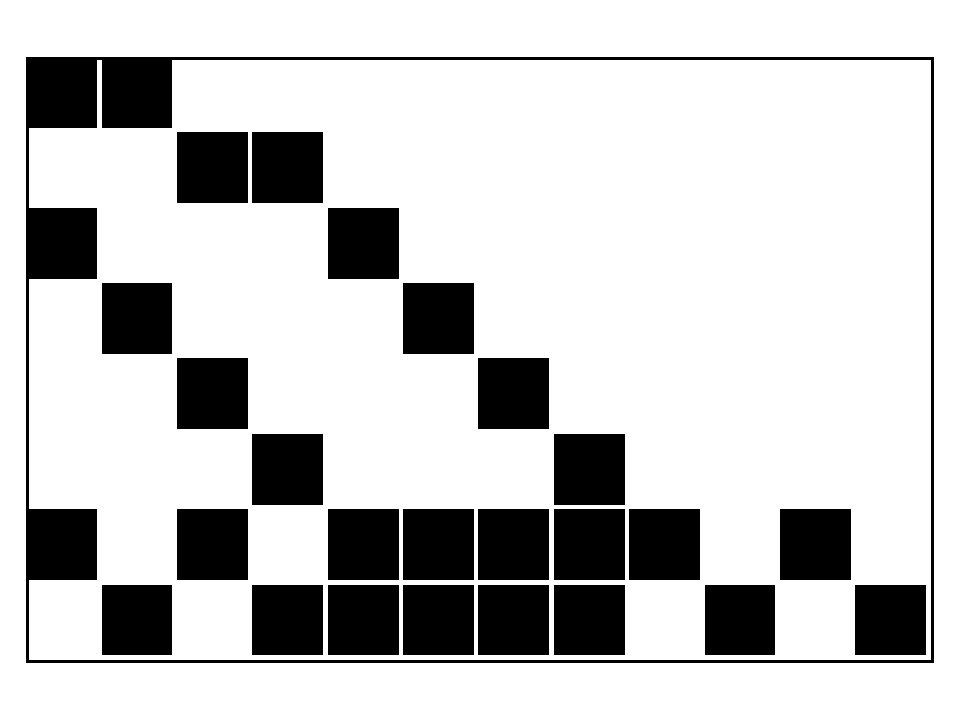
\includegraphics[width=0.85\linewidth]{AIRLIFT_1}
	\caption{CHEM\_1: Extensive form constraint matrix plot}
	\label{fig:chem_sparsity}
\end{figure}

\subsubsection{\chem: Mathematical formulation}
Table \ref{chem:notation} summarizes the notation used to formulate \chem. Using the notation, the problem can be formulated by the following extensive form.
\begin{subequations} \label{chem:formulation}
	\begin{align}
	(\chem)\ \textrm{max}\ & -\sum_{t\in T}\left[ \sum_{r\in R}v_{rt}^\textrm{b}q_{rt}^\textrm{b} + \sum_{j\in J}\left( C_{jt}n_{j,t+\delta}+\sum_{i\in I}c_{ijt}^\textrm{o}y_{ijt} \right) \right] \nonumber \\ 
	&\qquad\qquad\qquad\qquad\qquad\qquad\qquad\qquad\quad+ \sum_{\sigma\in\mathcal{S}}\PP(\sigma)\sum_{t\in T}\sum_{r\in R} v_{rt\sigma}^{\textrm{s}}q_{rt\sigma}^{\textrm{s0}} \label{chem:obj}\\
%	&\qquad\qquad\qquad\qquad\qquad\qquad\qquad\qquad+\sum_{j\in R}\left( c_j^+ y_j^{+s}+c_j^- y_j^{-s} \right)\Bigg]\label{airlift:obj} \\
	\textrm{s.t.}\ & \sum_{i\in I_j^{\textrm{tasks}}}p_{ij}y_{ijt}\le H_t\sum_{\tau=1}^{t}n_{j\tau},\quad\forall j\in J,\ \forall t\in T,\label{chem:b}\\
	&\sum_{j\in J}\sum_{i\in I_j^{\textrm{tasks}}}c_{ijt}^\textrm{o} y_{ijt} \le C_t^\textrm{o}\sum_{j\in J}\sum_{\tau=1}^{t}n_{j\tau},\quad\forall t\in T, \label{chem:c} \\
	&A_{rt}=A_{r,t-1}+\sum_{i\in I_r^{\textrm{tasks,p}}}\sum_{j\in I_i^\textrm{equip}}f_{ri}^\textrm{p}B_{ijt}-\sum_{i\in I_r^{\textrm{tasks,c}}}\sum_{j\in I_i^\textrm{equip}}f_{ri}^\textrm{c}B_{ijt}\nonumber\\
	&\qquad\qquad\qquad\qquad\qquad\qquad\qquad\quad\quad  -q_{rt}^\textrm{s}+q_{rt}^\textrm{b},\quad\forall r\in R,\ \forall t\in T,\label{chem:d}\\
	&A_{rt}\le A_{rt}^\textrm{max},\quad\forall r\in R,\ \forall t\in T,\label{chem:e}\\
	&B_{ijt}\le m_{ij}y_{ijt},\quad\forall i\in I,\ \forall j\in J,\ \forall t\in T,\label{chem:f}\\
	&q_{rt}^\textrm{b}\le Q_{rt}^\textrm{b},\quad\forall r\in R,\ \forall t\in T,\label{chem:i}\\
	&q_{rt}^\textrm{s}=q_{rt\sigma}^{\textrm{s0}}+q_{rt\sigma}^{\textrm{s+}},\quad\forall r\in R,\ \forall t\in T,\ \forall \sigma\in\mathcal{S},\label{chem:g}\\
	&q_{rt\sigma}^\textrm{s0}\le Q_{rt\sigma}^\textrm{s},\quad\forall r\in R,\ \forall t\in T,\ \forall \sigma\in\mathcal{S},\label{chem:h}\\
	&\sum_{j\in J}C_{jt}n_{jt}+\sum_{r\in R}v_{rt}^\textrm{b}q_{rt}^\textrm{b}\le MC_t,\quad\forall t\in T,\label{chem:j}\\
	&x_{t\sigma}=\left\{ 
				\begin{array}{ll}
					1& \textrm{if for each $r$, $q_{rt\sigma}^\textrm{s0}=Q_{rt\sigma}^\textrm{s}$,}\\ 
					0& \textrm{otherwise,}
				\end{array}	
			\right. \quad\forall t\in T,\ \forall \sigma\in\mathcal{S}, \label{chem:k}\\
	&\sum_{\sigma\in\mathcal{S}}x_{t\sigma}\ge G_t,\quad\forall t\in T,\label{chem:l}\\
	&\textrm{(First-stage variable bounds)} \nonumber\\	
	&A_{rt},q_{rt}^\textrm{b},q_{rt}^\textrm{s}\ge 0,\quad\forall r\in R,\ \forall t\in T,\label{chem:m}\\
	&B_{ijt}\ge 0,\quad\forall i\in I,\ \forall j\in J,\ \forall t\in T,\label{chem:n}\\
	&n_{jt}\in\mathbb{Z}_+,\quad\forall j\in J,\ \forall t\in T,\label{chem:o}\\
	&y_{ijt}\in\mathbb{Z}_+,\quad\forall i\in I,\ \forall j\in J,\ \forall t\in T,\label{chem:p}\\
	&\textrm{(Second-stage variable bounds)} \nonumber\\	
	&x_{t\sigma}\in \{0,1\},\quad \forall t\in T,\ \forall\sigma\in\mathcal{S},\label{chem:q}\\
	&q_{rt\sigma}^\textrm{s0},q_{rt\sigma}^\textrm{s+}\ge 0,\quad\forall r\in R,\ \forall t\in T,\ \forall \sigma\in\mathcal{S}.\label{chem:r}
	\end{align}
\end{subequations}
The objective function (\ref{chem:obj}) maximizes the total profit from operating the chemical plants. Constraint (\ref{chem:b}) restricts the operation times of equipment (or plant) does not exceed the length of time in each time period for each type of equipment. Constraint (\ref{chem:c}) guarantees the total operating expense does not exceed the total operating budget. Constraints (\ref{chem:d}) and (\ref{chem:e}) the material balance on the systems that includes inventory, production, consumption, sales, and purchasing. Constraint (\ref{chem:f}) corresponds to the relationship between the total processed amount of task and the amount of output from the processing. Constraints (\ref{chem:g}) and (\ref{chem:j}) restrict the purchasing of each resource. Constraint (\ref{chem:h}) denotes a simple balance for the amount of resources to be sold. Constraint (\ref{chem:i}) restricts the maximum amount of resources to be sold which is lower than the demand level. Constraint (\ref{chem:k}) defines the indicator variable which is 1 if the demand be met exactly, 0 otherwise. Constraint (\ref{chem:l}) guarantees the minimum number of scenarios for which the demand may be met exactly. Finally, constraints (\ref{chem:m})-(\ref{chem:r}) restrict the space where the decision variables can take values from.
\begin{table}[H]
	\caption{Notations for \chem}
	\label{chem:notation}
	\resizebox{\textwidth}{!}
	{
		%		{@{}llp{3in}}
		\begin{tabular}{ll}
			\toprule
			\multicolumn{2}{l}{\textbf{Index sets:}} \\
			$I$ & index set of tasks ($i\in I$)\\ 
			$J$ & index set of equipment types ($j\in J$)\\ 
			$R$ & index set of resources ($r\in R$)\\ 
			$T$ & index set of time periods ($t\in T$)\\ 
			$\mathcal{S}$ & index set of scenarios ($\sigma\in \mathcal{S}$)\\
			$I_j^{\textrm{tasks}}$ & index set of tasks which can be processed in equipment $j$\\ 
			$I_i^{\textrm{equip}}$ & index set of equipment types which can process task $i$\\ 			
			$I_{r}^{\textrm{tasks,p}}$ & index set of tasks which produce resource $r$\\ 
			$I_{r}^{\textrm{tasks,c}}$ & index set of tasks which consume resource $r$\\
			\midrule
			\multicolumn{2}{l}{\textbf{Parameters:}} \\
			$C_{jt}$ & cost of purchasing an equipment type $j$ for subsequent use \\
			$H_t$ & length of stage $t$\\
			$v_{rt}^\textrm{b}$ & cost of resource when bought from suppliers $r$ at time $t$\\
			$v_{rt\sigma}^\textrm{s}$ & value of resource $r$ when sold to customers at time $t$ under scenario $\sigma$ \\		
			$p_{ij}$ & processing time of task $i$ in equipment type $j$\\
			$c_{ijt}^\textrm{o}$ & operating cost of task $i$ on equipment $j$ in time period $t$  \\
			$C_t^\textrm{o}$ & maximum available budget for time $t$\\
			$f_{ri}^{\textrm{p}}$ & fraction of resource $r$ produced in one unit of output of task $i$\\
			$f_{ri}^{\textrm{c}}$ & fraction of resource $r$ consumed in one unit of output of task $i$\\
			$m_{ij}$& amount of output from task $i$ on equipment $j$\\			
			$A_{rt}^{\textrm{max}}$& maximum amount of resource $r$ that can be stored at time $t$\\
			$Q_{rt}^\textrm{b}$ & maximum amount of resource $r$ which can be bought at time $t$ from external sources\\
			$Q_{rt\sigma}^\textrm{s}$ & maximum amount of resource $r$ which can be sold under scenario $\sigma$ at time $t$ for profit\\
			$MC_t$ & maximum budget investment that is allowed in time period $t$\\
			$G_t$ & minimum number of scenarios for which the demand may be met exactly \\
			$\delta$ & construction delay once the equipment has been ordered\\	
			$\PP(\sigma)$ & \textrm{the probability of occurence of scenario $\sigma$} \\ \midrule
			\multicolumn{2}{l}{\textbf{Decision variables:}} \\
			\textrm{(First-stage)} \nonumber\\
			$n_{jt}$ & number of new units of equipment type $j$ to come into the production line at time period $t$\\
			$A_{rt}$ & amount of resource $r$ in inventory at time $t$\\
			$B_{ijt}$ & total processed amount of task $i$ on equipment type $j$ during time $t$\\
			$y_{ijt}$ & number of times task $i$ is performed on equipment $j$ during time period $t$\\
			$q_{rt}^\textrm{b}$ & amount of resource $r$ bought at time $t$\\
			$q_{rt}^\textrm{s}$ & amount of resource $r$ sold at time $t$\\
			\textrm{(Second-stage)} \nonumber\\
			$x_{t\sigma }$ & 1 if demand be met exactly (i.e., $q_{rt\sigma}^{\textrm{s0}}=Q_{rt\sigma}^{\textrm{s}}$), 0 otherwise\\				
			$q_{rt\sigma}^\textrm{s0}$ & amount of resource $r$ produced and sold at time $t$ which is lower than the demand level under scenario $\sigma$ \\
			$q_{rt\sigma}^\textrm{s+}$ & amount of resource $r$ produced and sold at time $t$ which is above the demand level under scenario $\sigma$ \\
			\bottomrule
		\end{tabular}
	}
\end{table} 

\subsubsection{\chem: Data generation}
We use the same deterministic parameters that is provided by the original reference \cite{journal:SPR1994}: $|I|=4$, $|J|=3$, $|R|=7$, $|T|=2$. Since we neglect the operating costs ($c_{ijt}^\textrm{o}=0$) and the construction delay ($\delta=0$), constraints (\ref{chem:c}), (\ref{chem:j})-(\ref{chem:l}) do not need to be incorporated. 

For the stochastic parameters, unlike the original reference, we use uniform distributions that will generate the reasonable values compared to the probability distributions given in the reference.
%\begin{align*}
%\delta&=0,\\
%c_{ijt}^\textrm{o}&=0,\quad\forall i\in I,\ \forall j\in J,\ \forall t\in T,\\
%p_{ij}&=4,\quad\forall i\in I,\ \forall j\in J,\\
%f_{ri}^\textrm{p}&=f_{ri}^\textrm{c}=1,\quad\forall r\in R,\ \forall i\in I,\\
%m_{i1}&=100,\ m_{i2}=200,\ m_{i3}=150, \quad\forall i\in I,\\
%H_1&=H_2=80,\\
%A_{rt}^\textrm{max}&=400,\quad\forall r\in R,\ \forall t\in T,\\
%C_{11}&=2500,\ C_{12}=2600,\\
%C_{21}&=3000,\ C_{22}=3100,\\
%C_{31}&=2800,\ C_{32}=2900,\\
%v_{11}^\textrm{b}&=23,\ v_{12}^\textrm{b}=24,\\
%v_{21}^\textrm{b}&=25,\ v_{22}^\textrm{b}=26,\\
%Q_{1t}^\textrm{b}&=200,\quad\forall t\in T,\\
%Q_{2t}^\textrm{b}&=250,\quad\forall t\in T,\\
%\textrm{(Task-Equipment relationship)}&\\
%I_1^\textrm{tasks}&=I_2^\textrm{tasks}=\{1,4\},\\
%I_3^\textrm{tasks}&=\{2,3\},\\
%I_1^\textrm{equip}&=I_4^\textrm{equip}=\{1,2\},\\
%I_2^\textrm{equip}&=I_3^\textrm{equip}=\{3\},\\
%\textrm{(Resource-Task relationship)}&\\
%I_1^\textrm{tasks,p}&=I_2^\textrm{tasks,p}=\{\emptyset\},\\
%I_3^\textrm{tasks,p}&=\{1\},\\
%I_4^\textrm{tasks,p}&=I_5^\textrm{tasks,p}=\{2\},\\
%I_6^\textrm{tasks,p}&=\{3\},\\
%I_7^\textrm{tasks,p}&=\{4\},\\
%I_1^\textrm{tasks,c}&=\{1\},\\
%I_2^\textrm{tasks,c}&=\{1,3\},\\
%I_3^\textrm{tasks,c}&=\{2\},\\
%I_4^\textrm{tasks,c}&=\{\emptyset\},\\
%I_5^\textrm{tasks,c}&=\{3\},\\
%I_6^\textrm{tasks,c}&=\{4\},\\
%I_7^\textrm{tasks,c}&=\{\emptyset\}.
%\end{align*}

\begin{gather*}
\textbf{\textrm{(Deterministic parameters)}}\\
\delta=0,\\
c_{ijt}^\textrm{o}=0,\quad\forall i\in I,\ \forall j\in J,\ \forall t\in T,\\
p_{ij}=4,\quad\forall i\in I,\ \forall j\in J,\\
f_{ri}^\textrm{p}=f_{ri}^\textrm{c}=1,\quad\forall r\in R,\ \forall i\in I,\\
m_{i1}=100,\ m_{i2}=200,\ m_{i3}=150, \quad\forall i\in I,\\
H_1=H_2=80,\\
A_{rt}^\textrm{max}=400,\quad\forall r\in R,\ \forall t\in T,\\
C_{11}=2500,\ C_{12}=2600,\\
C_{21}=3000,\ C_{22}=3100,\\
C_{31}=2800,\ C_{32}=2900,\\
v_{11}^\textrm{b}=23,\ v_{12}^\textrm{b}=24,\\
v_{21}^\textrm{b}=25,\ v_{22}^\textrm{b}=26,\\
Q_{1t}^\textrm{b}=200,\quad\forall t\in T,\\
Q_{2t}^\textrm{b}=250,\quad\forall t\in T,\\
\textrm{(Task-Equipment relationship)}\\
I_1^\textrm{tasks}=I_2^\textrm{tasks}=\{1,4\},\\
I_3^\textrm{tasks}=\{2,3\},\\
I_1^\textrm{equip}=I_4^\textrm{equip}=\{1,2\},\\
I_2^\textrm{equip}=I_3^\textrm{equip}=\{3\},\\
\textrm{(Resource-Task relationship)}\\
I_1^\textrm{tasks,p}=I_2^\textrm{tasks,p}=\{\emptyset\},\\
I_3^\textrm{tasks,p}=\{1\},\\
I_4^\textrm{tasks,p}=I_5^\textrm{tasks,p}=\{2\},\\
I_6^\textrm{tasks,p}=\{3\},\\
I_7^\textrm{tasks,p}=\{4\},\\
I_1^\textrm{tasks,c}=\{1\},\\
I_2^\textrm{tasks,c}=\{1,3\},\\
I_3^\textrm{tasks,c}=\{2\},\\
I_4^\textrm{tasks,c}=\{\emptyset\},\\
I_5^\textrm{tasks,c}=\{3\},\\
I_6^\textrm{tasks,c}=\{4\},\\
I_7^\textrm{tasks,c}=\{\emptyset\}.\\
\textbf{\textrm{(Stochastic parameters)}}\\
Q_{4t\sigma}^{\textrm{s}}=Unif(0,150),\quad\forall t\in T,\ \forall\sigma\in\mathcal{S},\\
Q_{7t\sigma}^{\textrm{s}}=Unif(0,200),\quad\forall t\in T,\ \forall\sigma\in\mathcal{S},\\
v_{4t\sigma}^{\textrm{s}}=Unif(50,60),\quad\forall t\in T,\ \forall\sigma\in\mathcal{S},\\
v_{7t\sigma}^{\textrm{s}}=Unif(70,80),\quad\forall t\in T,\ \forall\sigma\in\mathcal{S}.
\end{gather*}


\subsection{\dcap: Dynamic capacity planning with stochastic demand} \label{DCAP}
\dcap\ is the problem of determining a capacity expansion schedule for a set of resources, and the assignment of resource capacity to task with stochastic requirement over a multi-period planning horizon. We refer to the main reference \cite{journal:AG2004}.

Fig. \ref{fig:dcap_sparsity} shows the sparsity pattern presents in extensive form \dcap\ (single scenario).
\begin{figure}[H]
	\centering
	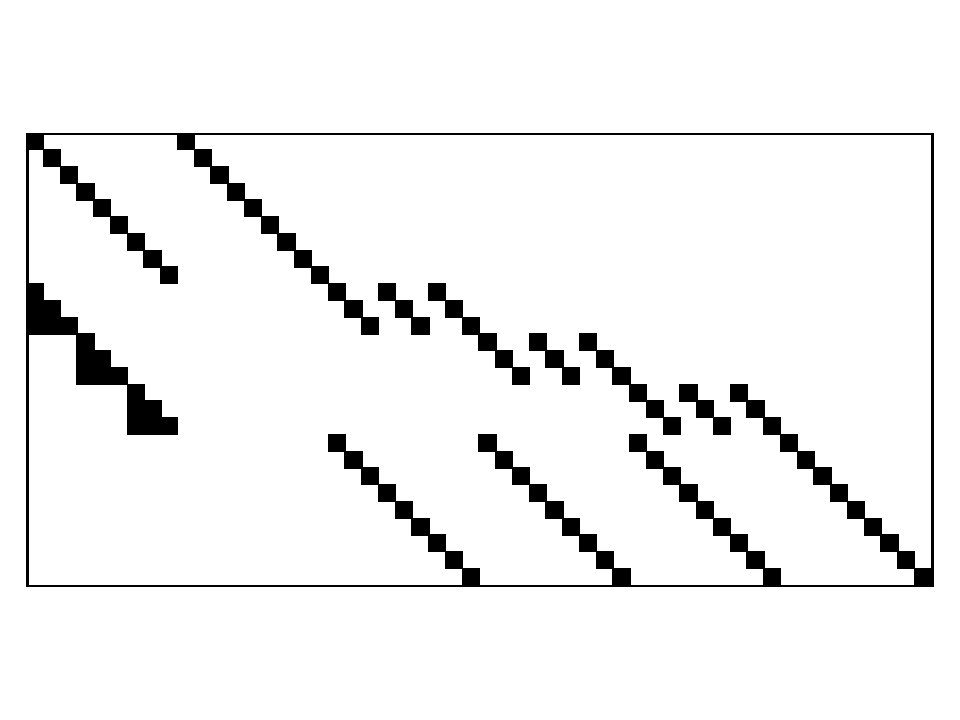
\includegraphics[width=\linewidth]{DCAP_3_3_3_1}
	\caption{DCAP\_3\_3\_3\_1: Extensive form constraint matrix plot}
	\label{fig:dcap_sparsity}
\end{figure}
%In \texttt{SIPLIB}, 12 instances are available in \texttt{SMPS} format with the largest instance comprises of 500 scenarios correspond to the size of 9,012 rows and 18,018 columns. 

%\dcap\ is a problem of deciding the capacity expansion schedule for $m$ resources over $T$ time periods in order to satisfy the processing requirements of $n$ tasks.
\subsubsection{\dcap: Mathematical formulation}
We consider the problem of deciding the capacity expansion schedule for $|R|$ resources over $|T|$ time periods to satisfy the processing requirements of $|N|$ tasks where $R$, $T$, and $N$ denote set of resources, set of time periods, and set of tasks, respectively. We define decision variables: the first-stage continuous variable $x_{it}$ for the capacity acquisition of resource $i$ in period $t$ and the second-stage binary variable $y_{ijt}^s$ to indicate whether resource $i$ is assigned to task $j$ in period $t$ under scenario $s$. Additional first-stage binary variable $u_{it}$ is for logical constraint whether or not we decided to acquire more capacity of resource $i$ in period $t$. Hence, for all resource $i\in R$ and time $t\in T$, $u_{it}=1$ if $x_{it}>0$, $u_{it}=0$ otherwise. 

Under the definition of the decision variables, the extensive form of \dcap\ is written below and the summarized notation is available in Table \ref{dcap:notation}.

\begin{subequations} \label{dcap:formulation}
	\begin{align}
	(\dcap)\ \textrm{min}\ &\sum_{t\in T}\sum_{i\in R}\left(\alpha_{it}x_{it}+\beta_{it}u_{it}\right)+\sum_{s\in\mathcal{S}}\PP(s)\sum_{t\in T}\sum_{i\in R\cup\{0\}}\sum_{j\in N}c_{ijt}^{s}y_{ijt}^s	\label{dcap:obj} \\
	\textrm{s.t.}\ & x_{it}\le \textrm{M}u_{it},\quad\forall i\in R,\ \forall t\in T,	\label{dcap:b}\\
	&\sum_{j\in N}d_{jt}^s y_{ijt}^s\le\sum_{\tau=1}^{t}x_{i\tau},\quad\forall i\in R,\ \forall t\in T,\ \forall s\in\mathcal{S},\label{dcap:c}\\
	&\sum_{i\in R\cup \{0\}}y_{ijt}^s=1,\quad\forall j\in N,\ \forall t\in T,\ \forall s\in\mathcal{S}, \label{dcap:d} \\
	&x_{it}\ge 0,\quad\forall i\in R,\ \forall t\in T,\label{dcap:e} \\
	&u_{it}\in\{0,1\}, \quad\forall i\in R,\ \forall t\in T,\label{dcap:f}\\
	&y_{ijt}^s\in\{0,1\},\quad\forall i\in R\cup\{0\},\ \forall j\in N,\ \forall t\in T,\ \forall s\in\mathcal{S},\label{dcap:g}
	\end{align}
\end{subequations}
The objective function (\ref{dcap:obj}) is to minimize total expected cost for the capacity expansion schedule. The first double summation denotes the expansion cost for resource $i$ in period $t$ where $\alpha_{it}$ and $\beta_{it}$ are the variable and fixed cost, respectively. The second term in the objective function represents the expected assignment cost in period $t$ over all scenario $s\in\mathcal{S}$. Note that a dummy resource $i=0$ is included with infinite capacity. The cost $c_{0jt}^s$ denotes the penalty of failing to assign a resource to task $j$. The dummy resource enforces the \textit{complete recourse property}, which ensures that there is a feasible second-stage assignment in all periods and all scenarios for any capacity acquisition schedule \cite{journal:AG2004}. Constraint (\ref{dcap:b}) is the logical constraint containing a suitably large value M (we set M=1 in \siplibtwo\ to follow the original implementation in \siplib\, although it does not seem to be large enough) to define the cost for capacity expansion. Constraint (\ref{dcap:c}) reflects that the processing requirement of all tasks assigned to a resource in any period cannot exceed the installed capacity in that period under all scenarios. Constraint (\ref{dcap:d}) guarantees that each task needs to be assigned to exactly one resource in each period under all scenarios. Finally, constraints (\ref{dcap:e})-(\ref{dcap:g}) restrict the space from which the variables take values.

\begin{table}[H]
	\caption{Notations for \dcap}
	\label{dcap:notation}
	\resizebox{\textwidth}{!}
	{
		\begin{tabular}{ll}
			\toprule
			\multicolumn{2}{l}{\textbf{Index sets:}} \\
			$R$ & index set of resources ($i\in R\cup\{0\}$ where $0$ is a dummy resource with infinite capacity) \\ 
			$N$ & index set of tasks ($j\in N$)\\ 
			$T$ & index set of time periods ($t\in T$)\\
			$\mathcal{S}$ & index set of scenarios ($s\in \mathcal{S}$) \\ \midrule
			\multicolumn{2}{l}{\textbf{Parameters:}} \\
			$\alpha_{it}$ & variable cost for expanding capacity of resource $i$\\ 
			$\beta_{it}$ & fixed cost for expanding capacity of resource $i$ \\ 
			$c_{ijt}^{s}$ & cost of processing task $j$ using resource $i$ in period $t$ under scenario $s$ \\ 
			$d_{jt}^s$	& processing requirement for task $j$ in period $t$ under scenario $s$		\\
			$\PP(s)$ & \textrm{the probability of occurence of scenario $s$} \\ \midrule
			\multicolumn{2}{l}{\textbf{Decision variables:}} \\
			$x_{it}$ (1st-stage) & capacity acquisition amount of resource $i$ in period $t$ \\ 
			$u_{it}$ (1st-stage)& 1 if capacity of resource $i$ is expanded in period $t$, 0 otherwise \\ 
			$y_{ijt}^s$ (2nd-stage)& 1 if resource $i$ is assigned to task $j$ in period $t$ under scenario $s$, 0 otherwise\\
			\bottomrule
		\end{tabular}
	}
\end{table} 

\subsubsection{\dcap: Data generation} \label{subsubsec:dcap_data_gen}
There are four factors that define the instance of \dcap: $|R|$, $|N|$, $|T|$, and $|\mathcal{S}|$. Once we decide the factors, the instance is named by DCAP\_$|R|$\_$|N|$\_$|T|$\_$|\mathcal{S}|$. Let $U$ be a continuous uniform random variable: $U\sim Unif(0,1)$. Then, the parameters are generated as follows:
\begin{align*}
	\alpha_{it}&=5U+5,\quad\forall i\in R,\ \forall t\in T, \\
	\beta_{it} &=40U+10,\quad\forall i\in R,\ \forall t\in T, \\
	c_{ijt}^s  &=5U+5,\quad\forall i\in R,\ \forall j\in N,\ \forall t\in T,\ \forall s\in\mathcal{S}, \\
	c_{0jt}^s  &=500U+500,\quad\forall j\in N,\ \forall t\in T,\ \forall s\in\mathcal{S}, \\
	d_{jt}^s   &=U+0.5,\quad\forall j\in N,\ \forall t\in T,\ \forall s\in\mathcal{S}.
\end{align*}

\subsection{\mptsps: Mutli-path traveling salesman problem with stochastic travel times} \label{MPTSPs}
\mptsps\ is a variant of the travelling salesman problem (TSP) where a set of paths exists between any two nodes and each path is characterized by a random travel time. 

In \siplib, only limited data (e.g., number of nodes, coordinates of nodes, generated travel times) are provided and no \smps\ file is available. We mainly refer to \cite{journal:PGM2017} for deriving the mathematical formulation. Due to the malfunction of subtour breaking constraints in the reference model, we refer to another paper \cite{journal:LSD1990} to contain working subtour-breaking constraint.

Fig. \ref{fig:mptsps_sparsity} shows the sparsity pattern presents in extensive form \mptsps\ (single scenario).
\begin{figure}[]
	\centering
	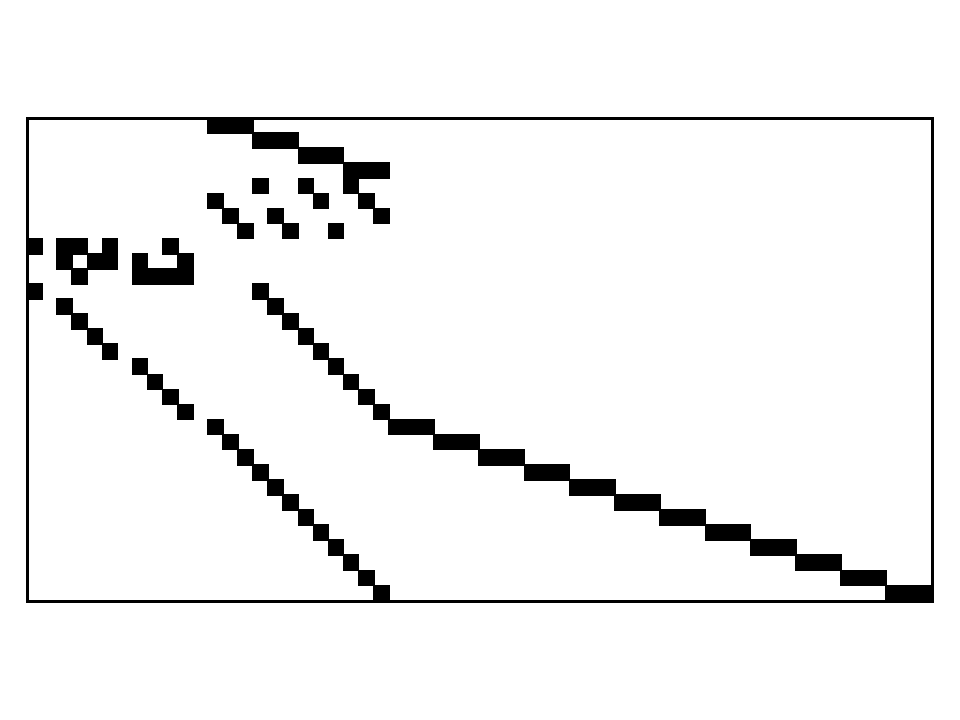
\includegraphics[width=\linewidth]{MPTSPs_D0_4_1}
	\caption{MPTSPs\_D0\_4\_1: Extensive form constraint matrix plot}
	\label{fig:mptsps_sparsity}
\end{figure}

 %Combining the two references, we construct the forthcoming single commodity flow-based formulation \mptsps\ that is used for \siplibtwo. 
\subsubsection{\mptsps: Mathematical formulation}
We consider a two-stage SIP with recourse. The travel time oscillation $e_{ij}^k$ by using path $k$ between nodes $i$ and $j$. We present each realization (scenario) of random travel time oscillation by $e_{ijk}^{s}$ where $s$ indicates the scenario. In \mptsps\, at the first stage, the decision-maker does not have any information about the travel time oscillation. The tour paths among the nodes, however, should be determined before the complete information is available. The first stage decision variable $y_{ij}$ is represented by the selection of nodes $i$ and $j$ to be visited in a tour. In the second stage where the random travel time $c_{ijk}^{s}$ are available, the paths $k$ between each couple of nodes $i$ and $j$ under scenario $s$, $x_{ijk}^{s}$ can be calculated. 

Let $N$ and $K_{ij}$, respectively, be the finite set of nodes of the graph and the set of paths between the pair of nodes $i,j\in N$. We denote with $\mathcal{S}$ the set of scenarios with associated equally distributed probability of each scenario $\PP(s)$, i.e., $\PP(s)\equiv 1/|\mathcal{S}|$. Each path $k\in K_{ij}$ between nodes $i,j\in N$ is characterized by a non-negative estimation of the mean unit travel time $\bar{c}_{ij}$ and a non-negative unit random travel time $c_{ijk}^{s}$ under the scenario $s\in S$. Let $e_{ijk}^{s}\equiv c_{ijk}^{s}-\bar{c}_{ij}$ be the error on the travel time estimated for the path $k\in K_{ij}$ under time scenario $s\in S$.

The first stage binary variables $y_{ij}=1$ if node $j\in N$ is visited right after node $i\in N$, 0 otherwise. The second stage binary variables $x_{ijk}^{s}=1$ if path $k\in K_{ij}$ between nodes $i,j\in N$ is selected at the second stage, 0 otherwise. We have one more set of first stage variables $\phi_{ij}$ which is introduced to break the subtours \cite{journal:LSD1990}. The non-negative continuous variables $\phi_{ij}$ describe the flow of a single commodity to node 1 from every other nodes (without loss of generality, 1 is the starting node). 

The extensive form of \mptsps\ is as follows and the notations used are summarized in Table \ref{mptsps:notation}.
\begin{subequations} \label{mptsps:formulation}
	\begin{align}
	(\mptsps)\ \textrm{min}\ &\sum_{i\in N}\sum_{j\in N\backslash\{i\}}\bar{c}_{ij}y_{ij}+\sum_{s\in \mathcal{S}}\PP(s)\sum_{i\in N}\sum_{j\in N\backslash\{i\}}\sum_{k\in K_{ij}}e_{ijk}^{s}x_{ijk}^{s} \label{mptsps:obj} \\ 
	\textrm{s.t.}\ &\sum_{j\in N\backslash\{i\}}y_{ij}=1,\quad\forall i\in N, \label{mptsps:con1} \\ 
	&\sum_{i\in N\backslash\{j\}}y_{ij}=1,\quad\forall j\in N,\label{mptsps:con2} \\ 
	&\sum_{j\in N}\phi_{lj}-\sum_{i\in N\backslash\{1\}}\phi_{il}=1,\quad\forall l\in N\backslash\{1\}, \label{mptsps:con3}  \\ 
	&\phi_{ij}\le \left(|N|-1\right)y_{ij},\quad\forall i\in N\backslash\{1\},\ \forall j\in N\backslash\{i\}, \label{mptsps:con4} \\ 
	&\sum_{k\in K_{ij}}x_{ijk}^{s}=y_{ij},\quad\forall i\in N,\ \forall j\in N\backslash\{i\},\ \forall s\in \mathcal{S}, \label{mptsps:con5} \\ 
	&y_{ij}\in \{0,1\},\quad \forall i\in N,\ \forall j\in N\backslash\{i\}, \label{mptsps:con6} \\ 
	&\phi_{ij} \ge 0, \quad \forall i\in N\backslash\{1\},\ \forall j\in N. \label{mptsps:con7} \\
	&x_{ijk}^{s}\in\{0,1\},\quad\forall i\in N,\ \forall j\in N\backslash\{i\},\ \forall k\in K_{ij},\ \forall s\in \mathcal{S}, \label{mptsps:con8} 
	\end{align}
\end{subequations}
The first sum in the objective function (\ref{mptsps:obj}) represents the first stage travel cost, while the second sum represents the recourse action, consisting in choosing the best path $k\in K_{ij}$ under scenario $s\in\mathcal{S}$. The constraints (\ref{mptsps:con1}) and (\ref{mptsps:con2}) form the assignment constraints and ensure that each node is visited only once. Given the fixed values of $y_{ij}$, constraint (\ref{mptsps:con3}) and (\ref{mptsps:con4}) form a network flow problem, and therefore the $\phi_{ij}$ values will be integer. In case the solutions of the above formulation contain at least one subtour, the constraints (\ref{mptsps:con3}) and (\ref{mptsps:con4}) are violated. Moreover, no tour can exist that does not contain node 1 by the two constraints. For more explanation on the subtour breaking mechanism accompanied with rigorous proof, refer to \cite{GG1978}. The constraint (\ref{mptsps:con5}) guarantees that path $k$ between nodes $i$ and $j$ can be chosen at stage 2 only if nodes $i$ and $j$ were part of the tour fixed at stage 1. Finally, the constraints (\ref{mptsps:con6})-(\ref{mptsps:con8}) restrict the space from which the variables take values.

\begin{table}[H]
	\caption{Notations for \mptsps}
	\label{mptsps:notation}
	\resizebox{\textwidth}{!}
	{
		\begin{tabular}{ll}
			\toprule
			\multicolumn{2}{l}{\textbf{Index sets:}} \\
			$N$ & \textrm{index set of nodes ($i,j,l\in N$)} \\ 
			$K_{ij}$ & \textrm{index set of paths between nodes $i$ and $j$ ($k\in K_{ij}$)} \\ 
			$\mathcal{S}$ & \textrm{index set of scenarios ($s\in \mathcal{S}$)}\\ \midrule
			\multicolumn{2}{l}{\textbf{Parameters:}} \\
			$c_{ijk}^{s}$ & \textrm{unit random travel time of path $k$ between nodes $i,j$ under scenario $s$} \\ 
			$\bar{c}_{ij}$ & \textrm{estimation of the mean unit travel time (expectation of $c_{ijk}^{s}$ over all $s$ and $k$)} \\ 
			$e_{ijk}^{s}$ & \textrm{the error on the travel time on estimated for arc $(i,j)$ and path $k$ under scenario $s$} \\ 
			$\PP(s)$ & \textrm{the probability of occurence of scenario $s$} \\  \midrule
			\multicolumn{2}{l}{\textbf{Decision variables:}} \\
			$\phi_{ij}$ (1st-stage) & \textrm{the nonnegative real-valued flow on arc $(i,j)$}\\
			$y_{ij}$ (1st-stage)& \textrm{1 if path $k$ between nodes $i,j\in N$ is selected at the second-stage, 0 otherwise} \\  
			$x_{ijk}^{s}$ (2nd-stage) & \textrm{1 if node $j$ is visited just after node $i$, 0 otherwise} \\ 
			\bottomrule
		\end{tabular}
	}
\end{table} 


\subsubsection{\mptsps: Data generation} \label{mptsps:datagen}
We follow the scenario generation methods described through the references \cite{journal:MPT2014,journal:PGM2017,journal:TPP2017}. For \mptsps\, there are three mainly distinguished characteristics for each instance: the nodes partition strategy ($D\in\{D0,D1,D2,D3\}$, explanation on each strategy is forthcoming), the number of nodes ($|N|\in\{2,3,\ldots\}$), and the number of scenarios ($|\mathcal{S}|\in\{1,2,\ldots\}$). Another important charicteristic $|K_{ij}|\in\{1,2,3,\ldots\}$ is the number of paths for each edge which is fixed by 3 as a default following \cite{journal:TPP2017}. Once we decide $D$, $|N|$, and $|S|$ by, each instance is named by MPTSPs\_$D$\_$|N|$\_$|\mathcal{S}|$.

The nodes are distributed in a circle with radius equal to $r$ km. We use Cartesian coordinate system where the geometric center of the circle is $(r,r)$. The nodes are distinguished by two subsets: \textit{central} and \textit{suburban}. If the Euclidean distance between a node and the geometric center is less than or equal to the half of the radius ($r/2$), then the node is of \textit{central} type. Otherwise, if the Euclidean distance is greater than the half of the radius, the node is of \textit{suburban} type. Each arc between any two nodes $i$ and $j$ is either \textit{homogeneous} or \textit{heterogeneous}. If the two nodes are of the same type of node, i.e., both are \textit{central} or both are \textit{suburban}, the type of the arc is \textit{homogeneous}. Otherwise, the type of the arc is \textit{heterogeneous}. Later, the travel time of each path between two nodes are affected by the type of arc. 

The nodes are generated by one of the following distribution strategies:
\begin{itemize}
	\item $D0$: All the nodes are \textit{central}.
	\item $D1$: All the nodes are \textit{suburban}.
	\item $D2$: 3/4 of the nodes are \textit{central} and the remaining 1/4 are \textit{suburban}.
	\item $D3$: 1/2 of the nodes are \textit{central} and the remaining 1/2 are \textit{suburban}.
\end{itemize}

Given $D,|N|$ and $|\mathcal{S}|$, the next procedure can be summarized as follows:
\begin{enumerate}
	\item Generate $|N|$ nodes based on the predetermined strategy $D$. Then, the nodes are generated by acceptance-rejection procedure with uniform random number generation. Again following \cite{journal:TPP2017}, we fix $r=7$\textit{km}. 
	\item Calculate Euclidean distances between the nodes ($EC_{ij}$).
	\item We guess and fix the deterministic velocity profile by 40\textit{km/h} for the \textit{central} nodes and 80\textit{km/h} for the \textit{suburban} nodes: $v_{cntr}=40$ and $v_{sbrb}=80$.
	\item Generate random travel times ($c_{ijk}^{s}$) for each scenario $s$.
	\begin{itemize}
		\item The velocity for traveling arc $(i,j)$ is affected by its arc type.
		%\item Each arc has $|K_{ij}|$ paths (we have fixed it $|K_{ij}|=3$ for all $i,j$).
		\item If the arc is \textit{homogeneous}, the random travel time of all the paths are generated only based on the corresponding velocity profile.
		\item If the arc is \textit{heterogeneous}, $\ceil*{\frac{|K_{ij}|}{3}}$ paths are generated based on $v_{cntr}=40$ and the remaining paths are generated based on $v_{sbrb}=80$. 
		\item The velocities are distributed by $Unif(\frac{v}{2},2v)$ for $v=v_{cntr},v_{sbrb}$.
		\item In summary, if the arc $(i,j)$ is \textit{homogeneous}, 
		\begin{align*}
		c_{ijk}^{s}\sim\left\{ \begin{array}{ll} \frac{EC_{ij}}{Unif(\frac{v_{cntr}}{2},2v_{cntr})} & \textrm{if $i,j$ are both \textit{central},} \\
		\frac{EC_{ij}}{Unif(\frac{v_{sbrb}}{2},2v_{sbrb})} & \textrm{if $i,j$ are both \textit{suburban},}	\end{array} \right.\ \forall k\in K_{ij}.
		\end{align*}
		\item Otherwise, if $(i,j)$ is \textit{heterogeneous},
		\begin{align*}
		c_{ijk}^{s}\sim\left\{ \begin{array}{ll} \frac{EC_{ij}}{Unif(\frac{v_{cntr}}{2},2v_{cntr})} & \textrm{for $k\in\left\{1,\ldots,\ceil*{\frac{|K_{ij}|}{3}}\right\}$,} \\
		\frac{EC_{ij}}{Unif(\frac{v_{sbrb}}{2},2v_{sbrb})} & \textrm{for $k\in\left\{\ceil*{\frac{|K_{ij}|}{3}}+1,\ldots,|K_{ij}|\right\}$.}	\end{array} \right.
		\end{align*}
	\end{itemize}
	\item Finally, we multiply 3600 for each component of $c_{ijk}^{s}$ to convert the unit from \textit{hours} to \textit{seconds}.
\end{enumerate}

\subsection{\phone: Telecommunication network planning} \label{PHONE}
\phone\ is a planning problem associated with networks for private line services. A manager of a network decides where and how much to expand the network capacity under the demand uncertainty between any two nodes. The manager has a limited budget with which the expansion is not penalized. Usually networks are very interconnected so that there is often more than one route that can satisfy a demand.

Fig. \ref{fig:phone_sparsity} shows the sparsity pattern presents in extensive form \phone\ (single scenario).
\begin{figure}[H]
	\centering
	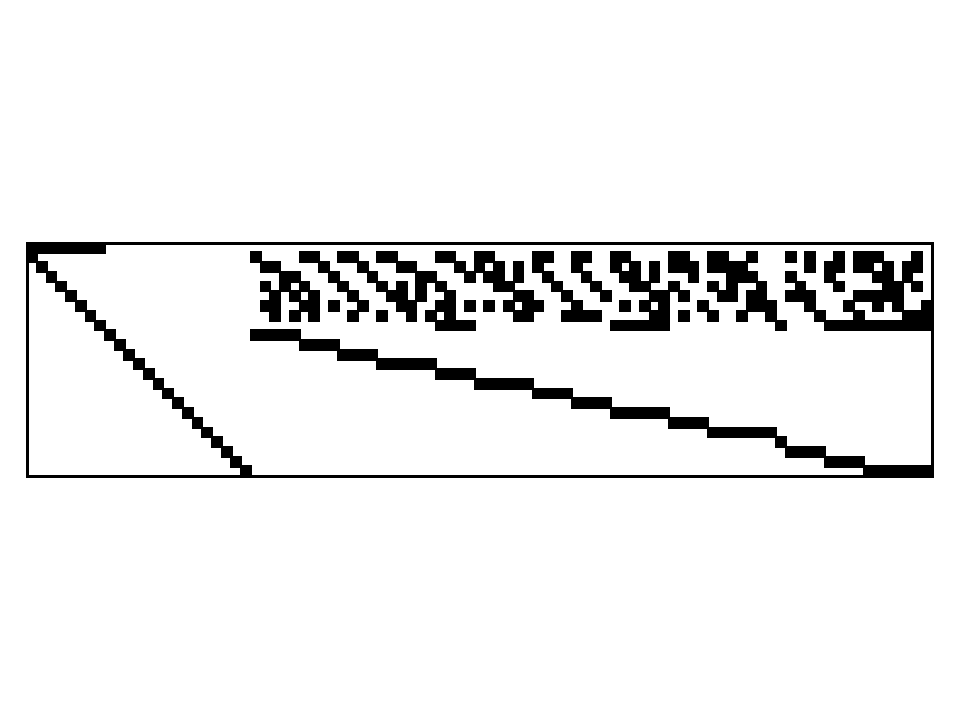
\includegraphics[width=\linewidth]{PHONE_1}
	\caption{PHONE\_1: Extensive form constraint matrix plot}
	\label{fig:phone_sparsity}
\end{figure}
\subsubsection{\phone: Mathematical formulation}
Table \ref{phone:notation} summarizes the notation used to formulate \phone. Using the notation, the problem can be formulated by the following extensive form.
\begin{subequations} \label{phone:formulation}
	\begin{align}
	(\phone)\ \textrm{min}\ &\sum_{s\in\mathcal{S}}\sum_{i\in P}u_i^s \label{phone:obj}\\
	\textrm{s.t.}\ &\sum_{j\in E} x_j \le b, \label{phone:b} \\
	&\sum_{i\in P} \sum_{r\in R(i)} a_{irj}f_{ir}^s\le x_j+e_j,\quad\forall j\in E,\ \forall s\in\mathcal{S},\label{phone:c}\\
	&\sum_{r\in R(i)}f_{ir}^s+u_i^s = d_i^s,\quad\forall i\in P,\ \forall s\in\mathcal{S}, \label{phone:d}\\
	&x_j\ge 0,\quad\forall j\in E, \label{phone:e}\\
	&u_{i}^s\ge 0,\quad\forall i\in P,\ \forall s\in\mathcal{S}, \label{phone:f}\\
	&f_{ir}^s\in\mathbb{Z}_+,\quad\forall i\in P,\ \forall r\in R(i),\ \forall s\in\mathcal{S}. \label{phone:g}
	\end{align}
\end{subequations}
The objective function (\ref{phone:obj}) minimizes the number of unserved requests. Constraint (\ref{phone:b}) stands for the budget limitation. Constraint (\ref{phone:c}) ensures that the number of connections serving pair $i$ must be less than the capacity. Constraint (\ref{phone:d}) means the sum of served and unserved requests equals to the original demands. Constraints (\ref{phone:e})-(\ref{phone:g}) define the range of the decision variables. 
\begin{table}[H]
	\caption{Notations for \phone}
	\label{phone:notation}
	\resizebox{\textwidth}{!}
	{
		\begin{tabular}{ll}
			\toprule
			\multicolumn{2}{l}{\textbf{Index sets:}} \\
			$P$ & index set of point-to-point pairs ($i\in P$) \\ 
			$E$ & index set of edges ($j\in E$) \\ 
			$R(i)$ & index set of routes to satisfy the requests between two points in pair $i$\\ 
			$\mathcal{S}$ & index set of scenarios ($s\in \mathcal{S}$)\\ \midrule
			\multicolumn{2}{l}{\textbf{Parameters:}} \\
			$b$ & total budget \\
			$a_{irj}$ & incidence parameter that is 1 if link $j\in R(i)$ for route $r$, 0 otherwise \\ 
			$e_j$ & the existing initial capacity in the network \\ 
			$d_{i}^s$ & the demands for service on pair $i$\\
			$\PP(s)$ & \textrm{the probability of occurence of scenario $s$} \\  \midrule
			\multicolumn{2}{l}{\textbf{Decision variables:}} \\
			$x_j$ (1st-stage) & the expanded capacity of link $j$\\
			$u_{is}$ (2nd-stage) & the number of unserved requests on point-to-point pair $i$ under scenario $s$\\  
			$f_{irs}$ (2nd-stage) & the number of connections serving point-to-point pair $i$ over route $r$ under scenario $s$\\ 
			\bottomrule
		\end{tabular}
	}
\end{table} 

\subsubsection{\phone: Data generation}
We adopt the numerical example provided in \cite{journal:AF2004}. The budget parameter $b$ is 3. The network comprises 6 nodes and 8 edges. Fig. \ref{fig:phone_network} shows the network structure with the initial capacity on each edge. We implement a recursive function to enumerate all possible routes for this example (see the function \texttt{allroutes()} in \texttt{Siplib/problems/PHONE/PHONE\_data.jl}).

Unlike the references, we use an uniform distribution: $Unif(5,15)$ for all the pairs to generate the uncertain demands.
\begin{figure}[H]
	\centering
	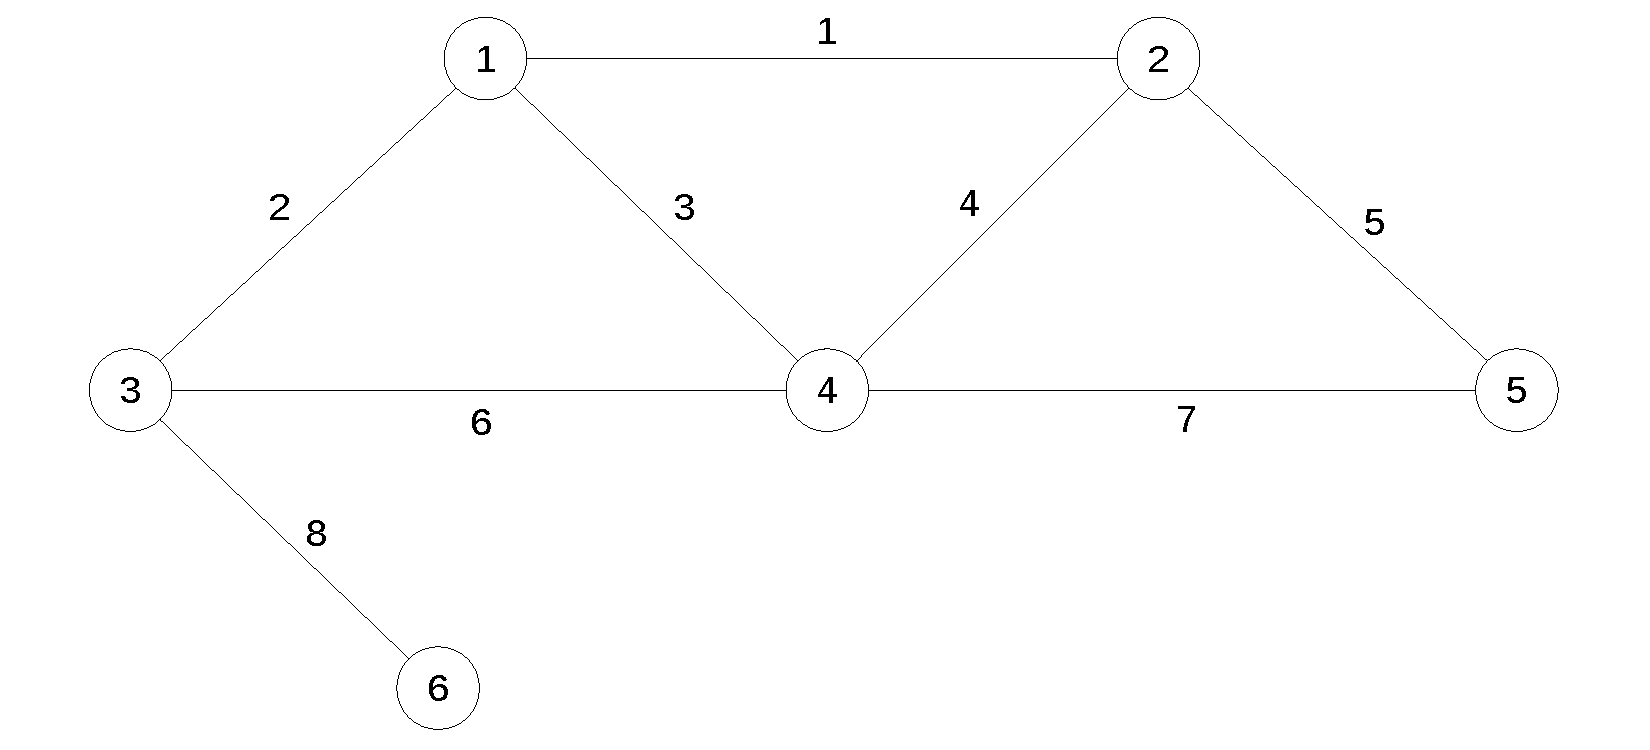
\includegraphics[width=\linewidth]{phone_network}
	\caption{Illustration of routing for telephone network example \cite{journal:AF2004}} 
	\label{fig:phone_network}
\end{figure}

\subsection{\sdcp: Stochastic data center placement} \label{SDCP}
The stochastic data center placement (SDCP) problem is to find the optimal placement of data centers (as dispatchable loads) that minimizes the expected total electricity dispatch cost over stochastic wind power generation scenarios. We refer to \cite{journal:KYZC2017} for mathematical models. For model parameters, we use Western Electricity Coordinating Council data set (WECC \cite{web:wecc}) interconnected with California ISO Open Access Same-Time Information System (CAISO) as in the reference. 

Fig. \ref{fig:sdcp_sparsity} shows the sparsity pattern presents in extensive form \sdcp\ (single scenario).
\begin{figure}[H]
	\centering
	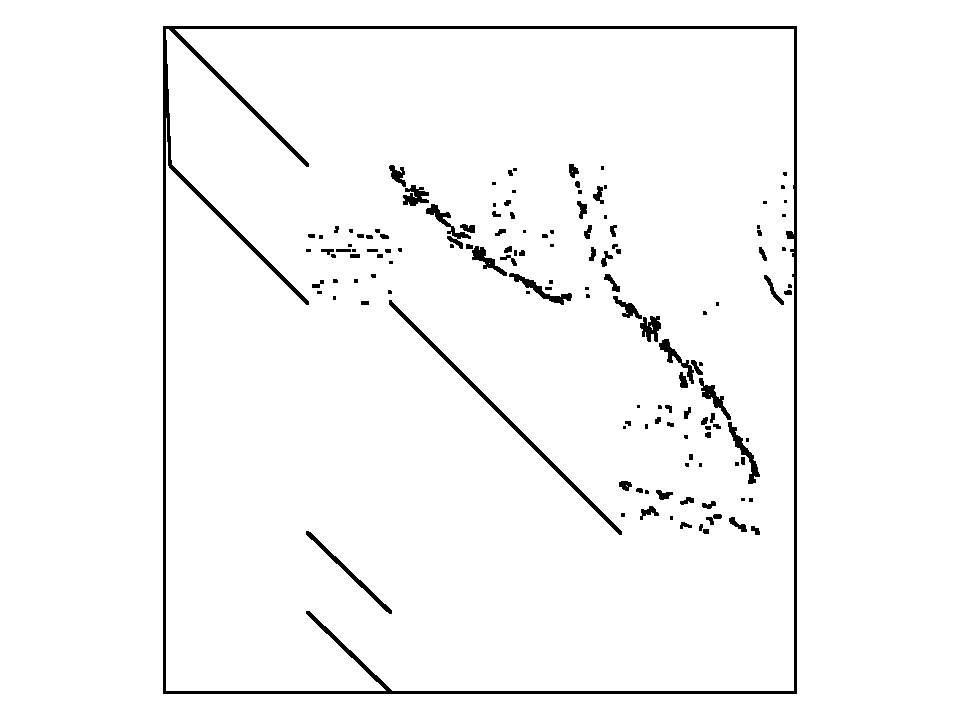
\includegraphics[width=\linewidth]{SDCP_5_10_FallWD_1}
	\caption{SDCP\_5\_10\_FallWD\_1: Extensive form constraint matrix plot}
	\label{fig:sdcp_sparsity}
\end{figure}

\subsubsection{\sdcp: Mathematical formulation}
In \sdcp, we make a here-and-now decision on the number and locations of data centers to be installed at location (bus) $n\in N$ at the first stage. In the second stage, the minimal cost recourse decision to dispatch loads and electricity is made considering wind power generation scenarios. The dispatching decision involves flows, angles, supply, loads, and spillages.

Using the notation in Table \ref{sdcp:notation}, the extensive form of \sdcp\ can be stated as in the following model \ref{sdcp:formulation}.
\begin{subequations} \label{sdcp:formulation}
	\begin{align}
	(\sdcp)\ \textrm{min}\ &\sum_{s\in\mathcal{S}}\PP(s)\sum_{t\in T} 
	\Bigg[\sum_{g\in G}C_g p_{gts} + \sum_{\lambda\in \mathcal{L}} C^{\mathcal{L}}x_{\lambda ts}^{\mathcal{L}} \nonumber \\&\qquad\qquad\qquad\qquad\qquad + \sum_{\iota\in \mathcal{I}} C^{\mathcal{I}}x_{\iota ts}^{\mathcal{I}} + \sum_{\rho\in \mathcal{R}} C^{\mathcal{R}}x_{\rho ts}^{\mathcal{R}} + \sum_{\omega\in \mathcal{W}} C^{\mathcal{W}}x_{\omega ts}^{\mathcal{W}} \Bigg]
	\label{sdcp:obj}\\
	\textrm{s.t.}\ &  \textrm{(First-stage constraints)} \nonumber\\
	&\sum_{n\in N} d_n \le K,\label{sdcp:b}\\
	&\textrm{(Second-stage constraints)} \nonumber\\
	&u_{nts} \le Ud_n,\quad\forall n\in N,\ \forall t\in T,\ \forall s\in\mathcal{S},\label{sdcp:c}\\
	&\sum_{l\in L_n^+}f_{lts}-\sum_{l\in L_n^-}f_{lts}+\sum_{g\in G_n}p_{gts}+\sum_{\iota\in IG_n^\mathcal{I}}\left(IC_{\iota t}^\mathcal{I}-x_{\iota ts}^\mathcal{I}\right)\nonumber\\
	&+\sum_{\omega\in IG_n^\mathcal{W}}\left(IC_{\omega ts}^\mathcal{W}-x_{\omega ts}^\mathcal{W}\right)
	+\sum_{\rho\in IG_n^\mathcal{R}}\left(IC_{\rho t}^\mathcal{R}-x_{\rho ts}^\mathcal{R}\right)
	-u_{nts} \nonumber\\
	&=\sum_{\lambda\in IG_n^\mathcal{L}}\left(IC_{\lambda t}^\mathcal{L}-x_{\lambda ts}^\mathcal{L}\right),\quad\forall n\in N,\ \forall t\in T,\ \forall s\in\mathcal{S},\label{sdcp:d}\\
	&f_{lts}=B_l\left(  \theta_{n_1 ts}-\theta_{n_2 ts}  \right),\quad\forall l\equiv (n_1, n_2)\in L,\ t\in T, s\in\mathcal{S},\label{sdcp:e}\\
	&-R_g^- \le p_{gts}-p_{g,t-1,s} \le R_g^+ ,\quad\forall g\in G,\ \forall t\in T,\ \forall s\in\mathcal{S},\label{sdcp:f}\\
	&  \textrm{(First-stage variable bounds)} \nonumber\\
	&d_n \in \mathbb{Z}_+,\quad \forall n\in N,\label{sdcp:g}\\
	&  \textrm{(Second-stage variable bounds)} \nonumber\\
	&u_{nts}\ge 0,\quad\forall n\in N,\ \forall t\in T,\ \forall s\in\mathcal{S},\label{sdcp:h}\\
	&-360\le\theta_{nts}\le 360,\quad\forall n\in N,\ \forall t\in T,\ \forall s\in\mathcal{S},\label{sdcp:i}\\
	&-TC_l\le f_{lts}\le TC_l,\quad\forall l\in L,\ \forall t\in T,\ \forall s\in\mathcal{S},\label{sdcp:j}\\
	&0\le p_{gts}\le P_g^+,\quad\forall g\in G,\ \forall t\in T\cup\{0\},\ \forall s\in\mathcal{S},\label{sdcp:k}\\
	&0\le x_{\lambda ts}^\mathcal{L}\le IC_{\lambda t}^\mathcal{L},\quad\forall \lambda\in \mathcal{L},\ \forall t\in T,\ \forall s\in\mathcal{S},\label{sdcp:l}\\
	&0\le x_{\iota ts}^\mathcal{I}\le IC_{\iota t}^\mathcal{I},\quad\forall \iota \in \mathcal{I},\ \forall t\in T,\ \forall s\in\mathcal{S},\label{sdcp:m}\\
	&0\le x_{\rho ts}^\mathcal{R} \le IC_{\rho t}^\mathcal{R},\quad\forall \rho\in\mathcal{R},\ \forall t\in T,\ \forall s\in\mathcal{S},\label{sdcp:n}\\
	&0\le x_{\omega ts}^\mathcal{W}\le IC_{\omega ts}^W,\quad\forall \omega\in\mathcal{W},\ \forall t\in T,\ \forall s\in\mathcal{S}.\label{sdcp:o}
	\end{align}	
\end{subequations}
The objective function (\ref{sdcp:obj}) is to minimize expected total dispatch costs. Constraints (\ref{sdcp:b}) is for the first-stage that represents the limitation of budget to install data centers. Constraint (\ref{sdcp:c}) sets the upper limit ($U$ for each data center) of the dispatchable loads from bus $n$. Constraint (\ref{sdcp:d}) guarantees the power flow balance of the network. Constraint (\ref{sdcp:e}) determines the best phase angle difference between two buses $n_1$ and $n_2$ on the line to minimize the power loss during transmission based on the Kirchhoff's law. Constraint (\ref{sdcp:f}) restricts ramping up/down capacity between two successive time slots. Constraints (\ref{sdcp:g})-(\ref{sdcp:o}) define the types and bounds for decision variables.

\begin{table}[H]
	\centering
	\caption{Notations for \sdcp}
	\label{sdcp:notation}
	\resizebox{\textwidth}{!}
	{
		\begin{tabular}{ll}
			\toprule
			\multicolumn{2}{l}{\textbf{Index sets:}} \\
			$\mathcal{S}$ & index set of scenarios ($s\in\mathcal{S}$) 		\\ 		
			$N$ & index set of all buses ($n\in N$)\\
			$T$ & index set of all time periods ($t\in T$)\\
			$L$ & index set of all transmission lines ($l\in L$) \\
			$\mathcal{L}$ & index set of all loads ($\lambda \in \mathcal{L}$)\\
			$\mathcal{I}$ & index set of all import points ($\iota\in \mathcal{I}$)\\
			$\mathcal{R}$ & index set of all non-wind renewable generators ($\rho\in \mathcal{R}$)\\
			$\mathcal{W}$ & index set of all wind generators ($\omega\in \mathcal{W}$)\\
			$G$ & index set of all generators ($g\in G$)\\
			\multicolumn{2}{l}{\textbf{(mapping sets)}} \\
			$G_n$ & index set of generators that are located in bus $n$ ($g\in G_n$)\\
			$IG_n^\mathcal{L}$ & index set of loads (or demand) that bus $n$ can supply ($\lambda\in IG_n^\mathcal{L}$)\\
			$IG_n^\mathcal{I}$ & index set of import points that can supply bus $n$ ($\iota\in IG_n^\mathcal{I}$) \\
			$IG_n^\mathcal{R}$ & index set of non-wind renewable generators that can supply bus $n$ ($\rho\in IG_n^\mathcal{R}$) \\
			$IG_n^\mathcal{W}$ & index set of wind generators that can supply bus $n$ ($\omega\in IG_n^\mathcal{W}$)\\
			$L_n^{+}$ & index set of outgoing transmission lines from bus $n$ ($l\in L_n^+$)\\
			$L_n^{-}$ & index set of incoming transmission lines to bus $n$ ($l\in L_n^-$)\\ \midrule
			\multicolumn{2}{l}{\textbf{Parameters:}} \\
			$\PP(s)$	&probability of occurence for scenario $s$\\
			$K$	& Maximum number of data centers \\
			$U$ & Dispatchable load capacity per data center \\
			\multicolumn{2}{l}{\textbf{(cost)}} \\
			$C_g$ & marginal generation cost of generator $g$	\\
			$C^\mathcal{L}$ & marginal load shedding cost of loads in $\mathcal{L}$	\\
			$C^\mathcal{I}$ & marginal spillage cost of import points in $\mathcal{I}$ \\
			$C^\mathcal{R}$ & marginal spillage cost of non-wind  renewable generators in $\mathcal{R}$ \\ 
			$C^\mathcal{W}$ & marginal spillage cost of wind generators in $\mathcal{W}$ \\
			\multicolumn{2}{l}{\textbf{(capacity)}} \\
			$B_{l}$ & susceptance of line $l$ under scenario $s$\\
			$TC_l$ & capacity of transmission line $l$\\
			$P_{g}^+$ & maximum generation capacity of generator $g$\\
			$R_{g}^+$ & ramping up capacity of generator $g$\\
			$R_{g}^-$ & ramping down capacity of generator $g$\\
			\multicolumn{2}{l}{\textbf{(supply/demand)}} \\
			$IC_{\lambda t}^\mathcal{L}$ & demand at load $\lambda$\\
			$IC_{\iota t}^\mathcal{I}$ & generation from import point $\iota$\\
			$IC_{\rho t}^\mathcal{R}$ & generation from renewable generator $\rho$\\
			$IC_{\omega ts}^\mathcal{W}$ & generation from wind generator $\omega$ under scenario $s$\\ \midrule
			\multicolumn{2}{l}{\textbf{Decision variables:}} \\
			$d_n$ (1st-stage) 	& (integer) number of dispatchable loads installed at bus $n$\\
			$u_{nts}$ (2nd-stage)	&	(continuous) load dispatching amount served at bus $n$ at time $t$ under scenario $s$\\
			$\theta_{gts}$ (2nd-stage)	&	(continuous) phase angle of generator $g$ at time $t$ under scenario $s$\\
			$f_{lts}$ (2nd-stage)	&	(continuous) power flow on line $l$ at time $t$ under scenario $s$\\
			$p_{gts}$ (2nd-stage)	&	(continuous) generation of generator $g$ at time $t$ under scenario $s$\\
			$x_{\lambda ts}^\mathcal{L}$	(2nd-stage) & (continuous) load shedding at load $\lambda$ at time $t$ under scenario $s$	\\
			$x_{\iota ts}^\mathcal{I}$	(2nd-stage) &	(continuous) spillage for import point $\iota$ at time $t$ under scenario $s$\\
			$x_{\rho ts}^\mathcal{R}$ (2nd-stage)	& (continuous) spillage for non-wind renewable generator $\rho$ at time $t$ under scenario $s$  	\\
			$x_{\omega ts}^\mathcal{W}$ (2nd-stage)	& (continuous) spillage for wind generator $\omega$ at time $t$ under scenario $s$ 	\\
			\hline
		\end{tabular}
	}
\end{table}

\subsubsection{\sdcp: Data generation}
Each \sdcp\ instance has four user-specifiable parameters: $K$, $P$, $D$, and $|\mathcal{S}|$. $K$ is the maximum number of installable data centers, $P$ is the wind penetration level (\%), $D$ is the season-day type which is one of FallWD, FallWE, WinterWD, WinterWE, SpringWD, SpringWE, SummerWD, SummerWE, and $|\mathcal{S}|$ is the number of scenarios. Once the four parameters are decided, the instance is named by SDCP\_$K$\_$P$\_$D$\_$|\mathcal{S}|$. For the default setting, we recommend to use $K=5$ and $P=10$.

For model parameters, we use a reduced model of the CAISO to follow the reference \cite{journal:KYZC2017}. The model includes a sparse representation of the entire WECC western interconnect outside of California. 
Based on the WECC, set cardinalities in \sdcp\ are as follows.
\begin{align*}
|N|&=225 \\
|T|&=24 \\
|L|&=375 \\
|\mathcal{L}|&=40\\
|\mathcal{I}|&=5\\
|\mathcal{R}|&=11\\
|\mathcal{W}|&=5\\
|G|&=130
\end{align*}

The marginal cost parameters for additional sources (load, import, non-wind renewable, wind) are fixed by
\begin{align*}
C^\mathcal{L}&=1000,\\
C^\mathcal{I}&=1000,\\
C^\mathcal{R}&=2000,\\
C^\mathcal{W}&=100.
\end{align*}
The dispatchable load capacity per data center ($U$) is fixed by 200 MWh.

Unlike other problems where stochastic data is generated while \julia\ script is running, we pre-generate and provide up to 1,000 wind power production profiles for each $D$ type. This data is included in ``\texttt{$\sim$/Siplib/src/problems/SCDP/data/WIND}'' folder and used to generate the stochastic wind data $IC_{\omega ts}^\mathcal{W}$. Hence, the number of scenarios that can be considered in an instance is limited to 1,000, which we think is large enough for computational experimental purpose.

\subsection{\sizes: Selection of an optimal subset of sizes} \label{SIZES}
\sizes\ is a simplified version of the cutting-stock problem with multi-period stochastic demand. We only consider the two-periods model to follow \cite{journal:JSW1999}. The first period demand is deterministic and the demand for the second period is stochastic. We refer to the mathematical formulation in \cite{journal:JSW1999} to construct \jumpmodel. Due to some unclear explanations (or typo), we slightly modify the formulation and use it for \siplibtwo.


Fig. \ref{fig:sizes_sparsity} shows the sparsity pattern presents in extensive form \sizes\ (single scenario).
\begin{figure}[H]
	\centering
	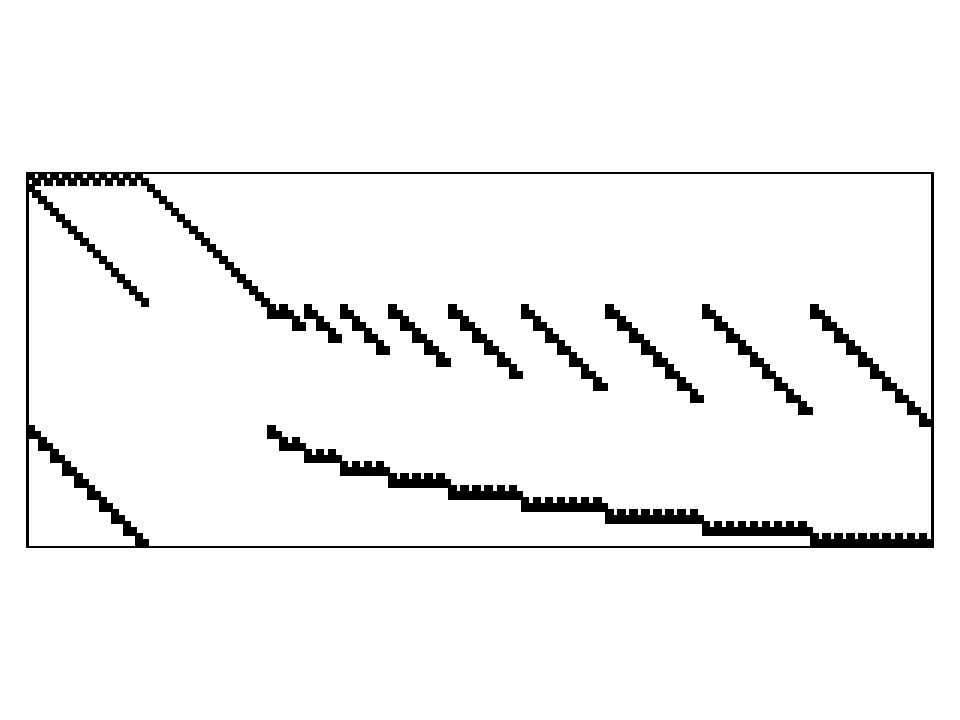
\includegraphics[width=\linewidth]{SIZES_1}
	\caption{SIZES\_1: Extensive form constraint matrix plot}
	\label{fig:sizes_sparsity}
\end{figure}
%In \siplib, only three instances are available in \smps\ files. 

\subsubsection{\sizes: Mathematical formulation}
Suppose a product is available in a finite number $|N|$ of sizes where 1 is the index of the smallest size and $|N|$ is the index of the largest size. Further, suppose size $i$ is substitutable for size $j$ if $i>j$, i.e., larger-sized items may fulfill demand for smaller sizes. Unlike typical cutting-stock problem, an item cannot be substituted into several pieces. 
Let $p_i$ be the unit production cost for size $i$. Generally $p_i>p_j$ for $i>j$. Let $f$ be the fixed setup cost for producing units of any size and $r$ be the unit penalty cost of meeting demand for size $j$ with a larger size $i$. Let $d_{jt}^s$ be the stochastic demand for size $j$ at time $t$ under scenario $l$. Let $c_t^l$ be the stochastic production capacity at time $t$ under scenario $s$. $\PP(s)$ is the equiprobable probability of occurence for scenario $s$.
We introduce three decision variables. The first-stage integer variable $y_{it}$ is the number of units of sizes $i$ produced at time $t$. Another first-stage variable $z_it$ is a binary variable that denotes whether or not we produce size $i$ item at time $t$ under scenario $l$. The second-stage integer variable $x_{ijt}^s$ denotes the number of units of size $i$ cut to meet demand for smaller size $j$ at time $t$ under scenario $s$. For $x_{ijt}^s$ with $i=j$, we use it to indicate that items of length index $i$ are to be used without cutting at time $t$ under scenario $s$.
Based on the above definitions, \sizes\ can be formulated by the following extensive form.

%\begin{subequations}
%	\begin{align}
%	(\texttt{SIZES})\ \textrm{min}\ &\sum_{t\in T}\sum_{i\in N} p_i y_{it} + \sum_{l\in \mathcal{L}} \PP(l)\sum_{t\in T}\left(\sum_{i\in N} sz_{it}^l+r\sum_{i\in N\backslash\{1\}}\sum_{j=1}^{i-1}x_{ijt}^l\right) \label{sizes:obj}\\
%	\textrm{s.t.}\ &\sum_{i\in N}y_{it}\le c_{t}^l,\quad \forall t\in T,\ \forall l\in \mathcal{L}, \label{sizes:b}\\
%	&\sum_{i=j}^{|N|} x_{ijt}^l \ge d_{jt}^l,\quad\forall j\in N,\ \forall t\in T,\  \forall l\in \mathcal{L},\label{sizes:c}\\
%	&\sum_{t'=1}^{t}\sum_{j=1}^{i}x_{ijt'}^l\le\sum_{t'=1}^{t}y_{it'}, \quad\forall i\in N,\ \forall t\in T,\ \forall l\in \mathcal{L},\label{sizes:d}\\
%	&y_{it}\le c_{t}^l z_{it}^l,\quad\forall i \in N,\ \forall t\in T,\ \forall l\in \mathcal{L},\label{sizes:e}\\
%	&y_{it}\in\mathbb{Z}_+,\quad \forall j\in N,\ \forall t\in T,\label{sizes:f}\\
%	&x_{ijt}^l\in\mathbb{Z}_+,\quad\forall i\in N,\ \forall j\in N,\ \forall t\in T,\ \forall l\in \mathcal{L},\label{sizes:g}\\
%	&z_{it}^l\in\{0,1\},\quad\forall i\in N,\ \forall t\in T,\ \forall l\in \mathcal{L}.\label{sizes:h}
%	\end{align}
%\end{subequations}

\begin{subequations} \label{sizes:formulation}
	\begin{align}
	(\sizes)\ \textrm{min}\ &\sum_{t\in T}\sum_{i\in N} \left(fz_{it} + p_i y_{it} \right) + 
	\sum_{s\in \mathcal{S}} \PP(s)\sum_{t\in T}\sum_{i\in N\backslash\{1\}}\sum_{j=1}^{i-1}rx_{ijt}^s \label{sizes:obj}\\
	\textrm{s.t.}\ &\sum_{i\in N}y_{it}\le c_{t},\quad \forall t\in T, \label{sizes:b}\\
	&y_{it}\le c_{t} z_{it},\quad\forall i \in N,\ \forall t\in T,\label{sizes:c}\\
	&\sum_{t'=1}^{t}\sum_{i=j}^{|N|} x_{ijt'}^s \ge d_{jt}^s,\quad\forall j\in N,\ \forall t\in T,\  \forall s\in \mathcal{S},\label{sizes:d}\\
	&\sum_{t'=1}^{t}\sum_{j=1}^{i}x_{ijt'}^s\le\sum_{t'=1}^{t}y_{it'}, \quad\forall i\in N,\ \forall t\in T,\ \forall s\in \mathcal{S},\label{sizes:e}\\
	&y_{it}\in\mathbb{Z}_+,\quad \forall j\in N,\ \forall t\in T,\label{sizes:f}\\
	&z_{it}\in\{0,1\},\quad\forall i\in N,\ \forall t\in T,\label{sizes:g}\\
	%&x_{ijt}^s\in\mathbb{Z}_+,\quad\forall i\in N,\ \forall j\in N,\ \forall t\in T,\ \forall s\in \mathcal{S}.\label{sizes:h} \\
	&x_{ijt}^s\in\mathbb{Z}_+,\quad\forall (i,j:i\ge j)\in N\times N,\ \forall t\in T,\ \forall s\in \mathcal{S}.\label{sizes:h}
	\end{align}
\end{subequations}

The first sum of the objective function (\ref{sizes:obj}) is the costs for producing items for all time periods (fixed + variable costs). The second term corresponds to the expectation of the penalty costs for substituting items. Constraint (\ref{sizes:b}) ensures the production for each period cannot exceed the capacity under all scenarios. Constraint (\ref{sizes:c}) is the logical constraint for the cost expression. (\ref{sizes:d}) guarantees the demand for each item can be met for all time periods and for all scenarios. Notice that constraint (\ref{sizes:d}) means the demand can be met by the items that are produced in the previous periods as well. Constraint (\ref{sizes:e}) enforces the supply limit. Constraints (\ref{sizes:f})-(\ref{sizes:h}) are binary or integer restrictions of the decision variables.

\begin{table}[H]
	\caption{Notations for \sizes}
	\label{sizes:notation}
	\resizebox{\textwidth}{!}
	{
		\begin{tabular}{ll}
			\toprule
			\multicolumn{2}{l}{\textbf{Index sets}} \\
			$N$ & \textrm{index set of items ($i,j\in N$)} \\ 
			$T$ & \textrm{index set of time periods ($t\in T$)} \\ 
			$\mathcal{S}$ & \textrm{index set of scenarios ($s\in\mathcal{S}$)}\\ \midrule
			\multicolumn{2}{l}{\textbf{Parameters}} \\
			$p_{i}$ & unit production cost for item $i$\\
			$f$	& fixed setup cost for producing any item\\
			$r$ & unit cutting cost\\ 
			$c_{t}$ & production capacity at time $t$\\
			$d_{it}^s$ &	demand for item $i$ at time $t$ under scenario $s$\\
			$\PP(s)$ & the probability of occurence of scenario $s$\\ \midrule
			\multicolumn{2}{l}{\textbf{Decision variables}} \\
			$y_{it}$ (1st-stage)  & number of units of size $i$ produced at time $t$ \\
			$z_{it}$ (1st-stage)& 1 if we produce size $i$ at time $t$, 0 otherwise\\
			$x_{ijt}^s$ (2nd-stage) & number of units of size $i$ cut to meet demand for smaller size $j$ at time $t$ under scenario $s$\\ 
			\bottomrule
		\end{tabular}
	}
\end{table} 

%\begin{table}[H]
%	\caption{Notations for \texttt{SIZES}}
%	\label{sizes:notation}
%	\resizebox{\textwidth}{!}
%	{
%		\begin{tabular}{ll}
%			\toprule
%			\multicolumn{2}{l}{\textbf{Index sets}} \\
%			$N$ & \textrm{index set of items ($i,j\in N$)} \\ 
%			$T$ & \textrm{index set of time periods ($t\in T$)} \\ 
%			$\mathcal{L}$ & \textrm{index set of scenarios ($l\in\mathcal{L}$)}\\ \midrule
%			\multicolumn{2}{l}{\textbf{Parameters}} \\
%			$d_{it}^l$ &	demand for item $i$ at time $t$ under scenario $l$\\
%			$p_{i}$ & unit production cost for item $i$\\
%			$s$	& setup cost for producing any item\\
%			$r$ & unit cutting cost\\ 
%			$c_{t}^l$ & production capacity at time $t$ under scenario $l$\\
%			$\PP(l)$ & the probability of occurence of scenario $l$\\ \midrule
%			\multicolumn{2}{l}{\textbf{Decision variables}} \\
%			$y_{it}$ ($1^{\textrm{st}}$ stage)  & number of units of size $i$ produced at time $t$ \\
%			$x_{ijt}^l$ ($2^{\textrm{nd}}$ stage) & number of units of size $i$ cut to meet demand for smaller size $j$ at time $t$ under scenario $l$\\ 
%			$z_{it}^l$ ($2^{\textrm{nd}}$ stage)& 1 if we produce size $i$ at time $t$ under scenario $l$, 0 otherwise\\
%			\bottomrule
%		\end{tabular}
%	}
%\end{table} 

\subsubsection{\sizes: Data generation}
Instances of \sizes\ are generated based on the one-period data given in Table \ref{sizes:data}. Note that although the table includes sleeve length data, we do not use this information for \sizes\ since this is not a typical cutting stock problem. Following \cite{journal:JSW1999}, we set the stochastic parameter $c_t^s=200,000$ to be deterministic for all $t\in T$ and $s\in\mathcal{S}$, hence only the demand parameter ($d_i^s$) is stochastic throughout the scenarios. The stochastic demand data is generated based on Table \ref{sizes:data}. First, we decide the number of scenarios to be generated by $|\mathcal{S}|$. Then, the demand data is specified by a vector of multipliers: one multiplier for each scenario that is multiplied times the demand vector from Table \ref{sizes:data}. For example, if $|\mathcal{S}|=3$, the instance is defined by $(0.7,1,1.3)$. Or if $|\mathcal{S}|=5$, the instance is defined by $(0.6,0.8,1,1.2,1.4)$. Since \siplib\ provides instances with $|\mathcal{S}|\le 20$, we recommend the users to use \siplibtwo\ to only generate instances with $|\mathcal{S}| \ge 20$. In \siplibtwo\, the multiplier vector is defined by the equally split set of subintervals between $[0.5,1.5]$, e.g., when $|\mathcal{S}|=20$, the multiplier vector is $(0.5,0.55,0.6,\ldots,1.4,1.45,1.5)$. With larger value of $|\mathcal{S}|$, we will have vector with finer granularity. To generate more random instances, the demand vector is multiplied by a continuous random number $U$ that is uniformly distributed in $(0.5,1.5)$. After that, the instance is named by SIZES\_$|\mathcal{S}|$.

\begin{table}[]
	\centering
	\caption{Base data for \sizes\ scenarios \cite{journal:JSW1999}}
	\label{sizes:data}
	\begin{tabular}{cccc}
		\hline
		$i$  & sleeve length & unit production cost ($p_i$) & demand ($d_i$) \\ \hline
		1  & 25            & 0.748                & 2500   \\
		2  & 30            & 0.7584               & 7500   \\
		3  & 35            & 0.7688               & 12500  \\
		4  & 40            & 0.7792               & 10000  \\
		5  & 45            & 0.7896               & 35000  \\
		6  & 50            & 0.8                  & 25000  \\
		7  & 55            & 0.8014               & 15000  \\
		8  & 60            & 0.8208               & 12500  \\
		9  & 65            & 0.8312               & 12500  \\
		10 & 70            & 0.8416               & 5000   \\ \hline
		\multicolumn{4}{c}{unit cutting cost ($u$): \$0.008}     \\
		\multicolumn{4}{c}{setup cost ($f$): \$453}              \\ 
		\multicolumn{4}{c}{production capacity ($c_t$): 200,000} \\ \hline
	\end{tabular}
\end{table}

\subsection{\smkp: Stochastic multiple knapsack problem} \label{SMKP}
\smkp\ is a class of stochastic multiple binary knapsack problems. Unlike typical knapsack problems where the objective is to maximize total profits under the restriction of the weight capacity of each knapsack, \smkp\ is to minimize total weights while satisfying a certain required profit for each knapsack. 

\siplib\ provides 30 instances of \smkp\ in total. The first-stage problems contain 240 binary variables and 50 knapsack constraints. The second-stage problems have 120 binary variables and 5 knapsack constraints. Each instance has 20 scenarios. 
We mainly refer to \cite{journal:AAD2014}.% for writing \texttt{Julia} script for \siplibtwo\ and explain the model throughout the following subsections.

Fig. \ref{fig:smkp_sparsity} shows the sparsity pattern presents in extensive form \smkp\ (single scenario).
\begin{figure}[H]
	\centering
	
\includegraphics[width=\linewidth]{SMKP_50_1}
	\caption{SMKP\_50\_1: Extensive form constraint matrix plot}
	\label{fig:smkp_sparsity}
\end{figure}

\subsubsection{\smkp: Mathematical formulation}
We have three types of items $x$, $z$, and $y$ where the first two types are of the first-stage and the last one is of the second-stage with stochastic scenarios. For each type, we have $|I|$ number of items where $I$ is the index set of the items. Hence, we define the binary variables $x_i$, $z_i$, and $y_i^s$ which are equal to 1 if the $i^{\mathrm{th}}$ item is decided to be included ($s$ denotes scenario so only appears in $y$-type variables). We consider two types of knapsacks: one associated with $x$-type and $z$-type items (say \texttt{xz}-knapsack) and the other one with $x$-type and $y$-type items (say \texttt{xy}-knapsack). \texttt{xz}-knapsacks are indexed by $j\in J$ and \texttt{xy}-knapsacks are indexed by $k\in K$.  Each knapsack has its own minimum level of profit that should be satisfied by the items of the associated types, e.g., the profit of the $j^{\mathrm{th}}$ \texttt{xz}-type knapsack is calculated based on the inclusion or exclusion of $x$-type and $z$-type items and should satisfy a certain requirement $b_j$. Bear in mind that the inclusion or exclusion of a certain item $i$ affects all the associated knapsacks.
 
Each parameter $c_i$, $d_i$, and $q_i^s$ denotes the gain of weight when including items of type $x$, $z$, and $y$, respectively. Here, $c_i$ and $d_i$ are deterministic and $q_i^s$ is stochastic. Parameters $a_{ji}$, $e_{ji}$, $t_{ki}$, and $w_{ki}$ are all deterministic and denote the profits for including items in the knapsacks. The RHS parameters $b_j$ and $h_k$ are the minimum levels of profit requirements for \texttt{xz}-knapsacks and \texttt{xy}-knapsacks, respectively.

The extensive form of \smkp\ is as follows and the notations used are summarized in Table \ref{smkp:notation}.
\begin{subequations} \label{smkp:formulation}
	\begin{align}
	(\smkp)\ \textrm{min}\ &\sum_{i \in I}\left(c_i x_i + d_i z_i\right) + \sum_{s\in\mathcal{S}}\PP(s)\sum_{i\in I}q_i^s y_i^s \label{smkp:obj}\\
	\textrm{s.t.}\ &  \sum_{i\in I}a_{ji}x_{i} + \sum_{i \in I}e_{ji}z_i\ge b_j,\quad\forall j\in J, \label{smkp:b}\\
	&  \sum_{i\in I} t_{ki}x_i + \sum_{i\in I}w_{ki} y_i^s\ge h_k,\quad\forall k\in K,\ \forall s\in\mathcal{S}, \label{smkp:c}\\
	&  x_i\in\{0,1\},\quad\forall i\in I, \label{smkp:d}\\
	&  z_i\in\{0,1\},\quad\forall i\in I, \label{smkp:e}\\
	&  y_i^s\in\{0,1\},\quad\forall i\in I,\ \forall s\in \mathcal{S}. \label{smkp:f}
	\end{align}
\end{subequations}

The objective (\ref{smkp:obj}) is to minimize the expected value of the total weights. Constraint (\ref{smkp:b}) ensures the minimum levels of profit requirements for all \texttt{xz}-knapsacks are satisfied. Constraint (\ref{smkp:c}) guarantees the minimum levels of profit requirements are satisfied for all \texttt{xy}-knapsacks under every scenario. Constraints (\ref{smkp:d})-(\ref{smkp:f}) are binary restriction of the decision variables.

\begin{table}[H]
	\caption{Notations for \smkp}
	\label{smkp:notation}
	\resizebox{\textwidth}{!}
	{
		\begin{tabular}{ll}
			\toprule
			\multicolumn{2}{l}{\textbf{Index sets:}} \\
			$I$ &  index set of items for each type ($i\in I$)\\ 
			$J$ &  index set of \texttt{xz}-knapsacks ($j \in J$)\\ 
			$K$ &  index set of \texttt{xy}-knapsacks ($k \in K$)\\
			$\mathcal{S}$ & index set of scenarios ($s\in \mathcal{S}$)\\ \midrule
			\multicolumn{2}{l}{\textbf{Parameters:}} \\
			$c_{i}$ 	& weight of the $i^{\mathrm{th}}$ $x$-type item 		\\ 
			$d_{i}$ 	& weight of the $i^{\mathrm{th}}$ $z$-type item  		\\ 
			$q_{i}^{s}$ & weight of the $i^{\mathrm{th}}$ $y$-type item under scenario $s$ 		\\ 
			$a_{ji}$	& profit of the $j^{\mathrm{th}}$ \texttt{xz}-knapsack for including $i^{\mathrm{th}}$ $x$-type item		\\
			$e_{ji}$	& profit of the $j^{\mathrm{th}}$ \texttt{xz}-knapsack for including $i^{\mathrm{th}}$ $z$-type item		\\
			$t_{ki}$	& profit of the $k^{\mathrm{th}}$ \texttt{xy}-knapsack for including $i^{\mathrm{th}}$ $x$-type item	\\
			$w_{ki}$	& profit of the $k^{\mathrm{th}}$ \texttt{xy}-knapsack for including $i^{\mathrm{th}}$ $y$-type item		\\
			$b_j$		& minimum required profit for the $j^{\mathrm{th}}$ \texttt{xz}-knapsack		\\
			$h_k$		& minimum required profit for the $k^{\mathrm{th}}$ \texttt{xy}-knapsack		\\
			$\PP(s)$ 	& \textrm{the probability of occurence of scenario $s$} \\ \midrule
			\multicolumn{2}{l}{\textbf{Decision variables:}} \\
			$x_{i}$ (1st-stage) & 1 if the $i^{\mathrm{th}}$ $x$-type item is decided to be included, 0 otherwise \\ 
			$z_{i}$ (1st-stage) & 1 if the $i^{\mathrm{th}}$ $z$-type item is decided to be included, 0 otherwise \\ 
			$y_{i}^s$ (2nd-stage)& 1 if the $i^{\mathrm{th}}$ $y$-type item is decided to be included under scenario $s$, 0 otherwise  \\
			\bottomrule
		\end{tabular}
	}
\end{table} 

\subsubsection{\smkp: Data generation}
There are two factors that define the instance of \smkp: $|I|$ and $|\mathcal{S}|$. The sizes for another sets are fixed by $|J|=50$ and $|K|=5$ following \cite{journal:AAD2014}. Once we decide the factors $|I|$ and $|\mathcal{S}|$, each instance is named by SMKP\_$|I|$\_$|\mathcal{S}|$. Again directly following \cite{journal:AAD2014}, we randomly generate the parameters. Let $U$ be a discrete uniform random variable: $U\sim Unif[1,100]$. Then, the parameters are generated as follows:
\begin{align*}
c_i		&=	U,\quad\forall i\in I, \\
d_i		&=	U,\quad\forall i\in I, \\
q_i^s	&= 	U,\quad\forall i\in I,\ \forall s\in\mathcal{S},\\
a_{ji}	&=	U,\quad\forall j\in J,\ \forall i\in I, \\
e_{ji}	&=	U,\quad\forall j\in J,\ \forall i\in I, \\
t_{ki}	&=	U,\quad\forall k\in K,\ \forall i\in I, \\
w_{ki}	&=	U,\quad\forall k\in K,\ \forall i\in I,  \\
b_j		&=	\frac{3}{4}\sum_{i\in I}\left(a_{ji}+e_{ji}\right),\quad\forall j\in J, \\
h_k		&=	\frac{3}{4}\sum_{i\in I}\left(t_{ji}+w_{ji}\right),\quad\forall k\in K. 
\end{align*}

\subsection{\sslp: Stochastic server location problem} \label{SSLP}
\sslp\ is a class of problem that finds the optimal location of servers and the optimal allocation of clients to servers which maximizes the expected net income under uncertain presents of clients. \sslp\ finds applications in a variety of domains such as network design for electric power, internet services, telecommunications, and water distribution. \siplib\ provides 12 instances with varying number of clients, server locations, and scenarios in \smps\ format. The largest instance includes 10 server locations, 50 clients, and 2,000 scenarios which corresponds to 120,001 constraints, 1,000,010 binary variables, and 20,000 continuous variables. We refer to \cite{journal:NS2005} for mathematical formulation and data generation forthcoming through the following subsections.

Fig. \ref{fig:sslp_sparsity} shows the sparsity pattern presents in extensive form \sslp\ (single scenario).
\begin{figure}[]
	\centering
	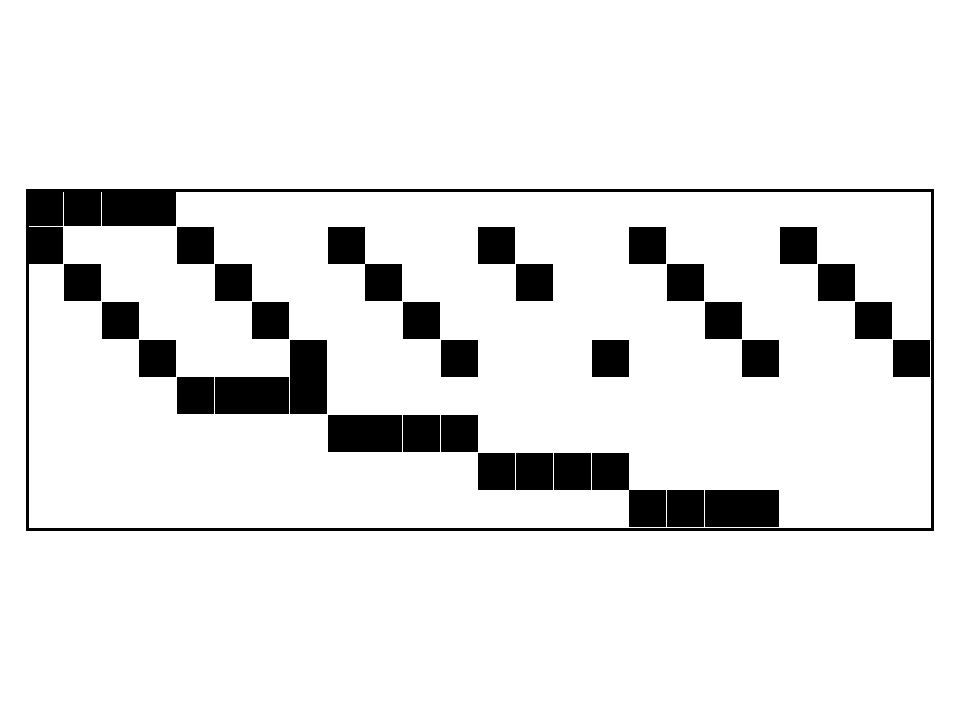
\includegraphics[width=\linewidth]{SSLP_4_4_1}
	\caption{SSLP\_4\_4\_1: Extensive form constraint matrix plot}
	\label{fig:sslp_sparsity}
\end{figure}

\subsubsection{\sslp: Mathematical formulation}
Let $I$, $J$, $Z$, and $\mathcal{S}$ be index sets for the clients, servers, zones, and scenarios. For $i\in I$, $j\in J$, $z\in Z$, and $s\in\mathcal{S}$, we define the notations in Table \ref{sslp:notation}.

Suppose that we place a server at location $j$. Then, the allocation costs $c_j$ and the server will provide capacity to serve up to $u$ amount of resource to clients. The revenue earned by serving client $i$ from location $j$ is denoted by $q_{ij}$. We have also a shortage cost (penalty) $q_{0j}$ for each unit of demand that remains unserved among the clients assigned to server $j$. If client $i$ is served by a server at location $j$, it uses $d_{ij}$ units of resource from the server. We allow only one server to be installed at each location and each client can only be served by one server. There is a requirement that a minimum number of servers to be located in a zone $z$, and is denoted by $w_z$. 

The first-stage binary variables $x_j$ decide whether or not a server is located at location $j$. The second-stage binary variables $y_{ij}^s$ are referred to as recourse decision under scenario $s$ and associated with the decision on serving client $i$ by server $j$. The variables $y_{ij}^s$ will be implemented in the future, when scenario $s$ is finally observed.

Based on the above, the extensive form of \sslp\ can be stated as follows:
\begin{subequations} \label{sslp:formulation}
	\begin{align}
	(\sslp)\ \textrm{min}\ &	\sum_{j\in J}c_j x_j - \sum_{s\in\mathcal{S}}\PP(s)\left(\sum_{i\in I}\sum_{j\in J}q_{ij}^s y_{ij}^s - \sum_{j\in J}q_{0j}^s y_{0j}^s \right) \label{sslp:obj} \\ 
	\textrm{s.t.}\ &\sum_{j\in J}x_j\le v,\label{sslp:b}\\ 
	&\sum_{j\in J_z}x_j\ge w_z,\quad\forall z\in Z,\label{sslp:c}\\
	&\sum_{i\in I}d_{ij}y_{ij}^s - y_{0j}^s\le ux_j,\quad\forall j\in J,\ \forall s\in\mathcal{S}, \label{sslp:d} \\
	&\sum_{j\in J}y_{ij}^s=h_i^s,\quad\forall i\in I,\ \forall s\in \mathcal{S}, \label{sslp:e}\\
	&x_j\in\{0,1\},\quad\forall j\in J,\label{sslp:f}\\
	&y_{ij}^s\in\{0,1\},\quad\forall i\in I,\ j\in J,\ s\in\mathcal{S}, \label{sslp:g}\\
	&y_{0j}^s\ge 0,\quad\forall j\in J,\ \forall s\in\mathcal{S} \label{sslp:h}.
	\end{align}
\end{subequations}
The objective function (\ref{sslp:obj}) is to maximize total expected revenue of locating servers and serving customers by the servers. Constraint (\ref{sslp:b}) satisfies the requirement that only up to a total of $v$ available servers can be installed. The zonal requirements that specify how many servers are needed in each zone are given by constraint (\ref{sslp:c}). Constraint (\ref{sslp:d}) ensures that a server located at site $j$ can serve only up to its capacity $u$. The variable $y_{0j}^s$ is introduced in the constraint (\ref{sslp:d}) to accomodate any overflows that are not served due to limitations in server capacity. These overflows result in a loss of revenue at a rate of $q_{0j}^s$. The inclusion of an artificial variable may allow a client to be assigned to servers that are not located. However, penalty costs associated with such an assignment may result in such high costs as to preclude it in an optimal solution, unless server capacity is so limited that some clients have to be turned away \cite{journal:NS2005}. Constraint (\ref{sslp:e}) guarantees that each client is served by only one server. Constraint (\ref{sslp:f}) and (\ref{sslp:g}) are binary restrictions on the decision variables. Finally, constraint (\ref{sslp:h}) is the non-negativity requirement on the overflow variables.
\begin{table}[H]
	\caption{Notations for \sslp}
	\label{sslp:notation}
	\resizebox{\textwidth}{!}
	{
		\begin{tabular}{ll}
			\toprule
			\multicolumn{2}{l}{\textbf{Index sets:}} \\
			$J$ 		  & index set of server locations ($j\in J$)\\ 
			$I$ 		  & index set of clients ($i\in I$)  \\ 
			$Z$ 		  & index set of zones ($z\in Z$) \\
			$\mathcal{S}$ & index set of scenarios ($s\in \mathcal{S}$)	\\ \midrule
			\multicolumn{2}{l}{\textbf{Parameters:}} \\
			$c_j$		& cost of locating a server at location $j$	\\
			$q_{ij}^s$	& revenue from client $i$ being served by server at location $j$ under scenario $s$	\\
			$q_{0j}^s$	& rate of revenue loss for overflows that are not served due to limited server capacity under scenario $s$	\\
			$d_{ij}$	& resource demand of client $i$ from server at location $j$	\\
			$u$			& server capacity	\\
			$v$			& upper bound on the total number of servers that can be located	\\
			$w_z$		& minimum number of servers to be located in zone $z$	\\
			$J_z$		& subset of server locations that belong to zone $z$	\\
			$h_i^s$		& 1 if client $i$ is present under scenario $s$, 0 otherwise	\\
			$\PP(s)$ 	& probability of occurence for scenario $s$\\ \midrule
			\multicolumn{2}{l}{\textbf{Decision variables:}} \\
			$x_j$ (1st-stage)  	 & 1 if a server is located at site $j$, 0 otherwise \\
			$y_{ij}^s$ (2nd-stage) & 1 if client $i$ is served by a server at location $j$ under scenario $s$, 0 otherwise\\
			$y_{0j}^s$ (2nd-stage) & non-negative amount of overflows that are not served due to the limitation on server $j$'s capacity	\\
			\bottomrule
		\end{tabular}
	}
\end{table} 

\subsubsection{\sslp: Data generation}
For each instance of \sslp\, we determine the number of potential server locations $|J|$, the number of clients $|I|$, and the number of scenarios $|\mathcal{S}|$. Then, the instance is named by SSLP\_$|J|$\_$|I|$\_$|\mathcal{S}|$. The client-server revenue are set to be 1 per unit of client demand. Some of deterministic parameters are randomly generated from the discrete uniform distribution while scenario data are generated from the Bernoulli distribution. In summary, the parameters are generated as follows:
\begin{align*}
c_j	&=Unif[40,80],\quad\forall j\in J,\\
d_{ij}	&= Unif[0,25],\quad\forall i\in I,\ \forall j\in J,\\
h_i^s	&= Bernoulli(0.5),\quad\forall i\in I,\ \forall s\in \mathcal{S},\\
q_{ij}^s	&= d_{ij},\quad\forall i\in I,\ \forall j\in J,\ \forall s\in\mathcal{S},\\
q_{0j}^s	&=	1000,\quad\forall j\in J,\ \forall s\in\mathcal{S},\\
v 		&= |J|	\\
u	&= \frac{3}{2}\times\frac{\sum_{i\in I}\sum_{j\in J}d_{ij}}{|J|} 
\end{align*}
Note that the zonal data is omitted due to the lack of available information. Hence, constraint (\ref{sslp:c}) does not appear in \siplibtwo\ instances. Note also that constraint (\ref{sslp:b}) is redundant since we set $v=|J|$. We include this redundant constraint to follow the former \siplib\ implementation although it seems like a bug.

\subsection{\suc: Stochastic unit commitment problem} \label{SUC}
The unit commitment (UC) problem is a production cost model (PCM) that plans power system operations over an extended time horizon. \suc\ is a stochastic version of UC for studying the impact of incorporating highly uncertain power generation of large-scale wind turbines with transmission constraints and system component failures. We refer to \cite{journal:PO2013} for mathematical models. For model parameters, we use Western Electricity Coordinating Council data set (WECC \cite{web:wecc}) interconnected with California ISO Open Access Same-Time Information System (CAISO) as in the reference. 

Fig. \ref{fig:suc_sparsity} shows the sparsity pattern presents in extensive form \suc\ (single scenario).
\begin{figure}[H]
	\centering
	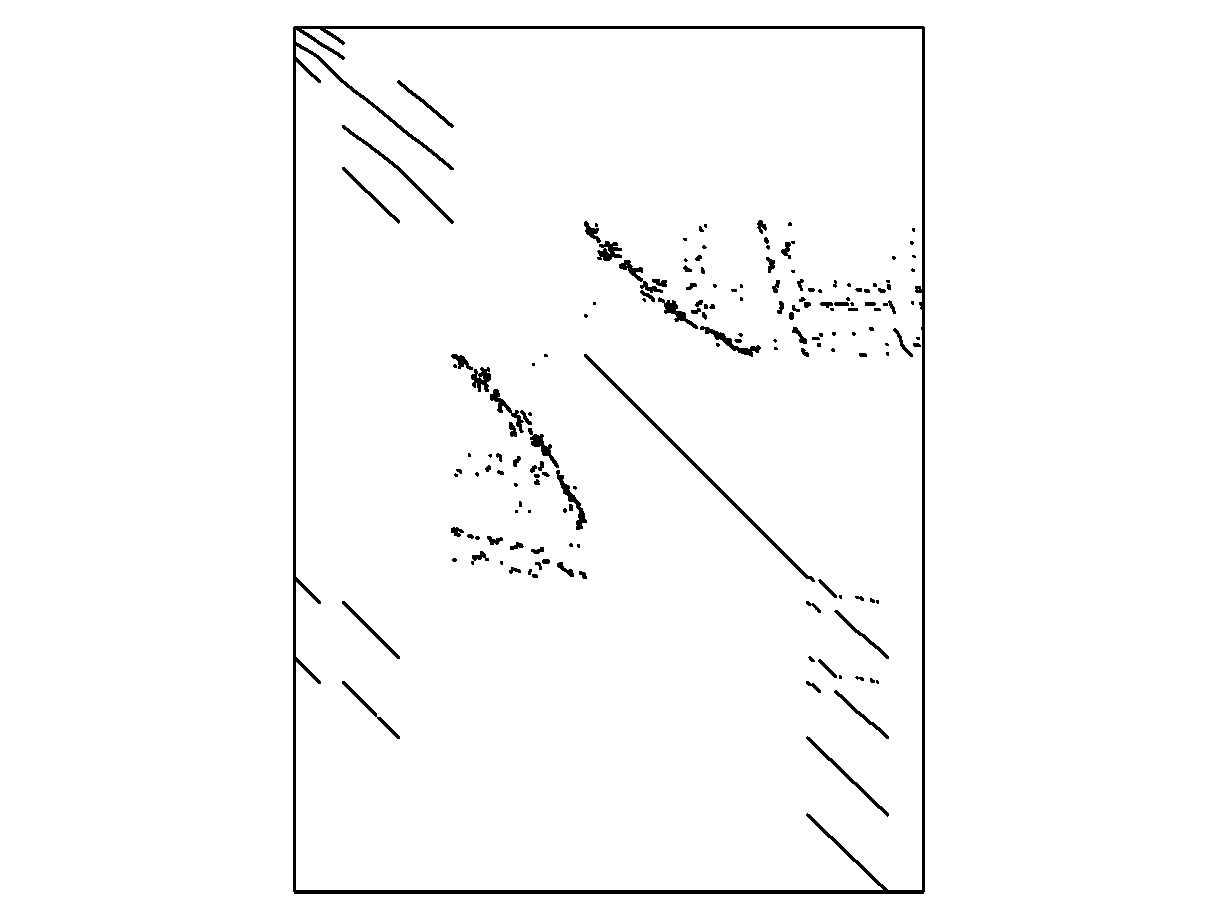
\includegraphics[width=\linewidth]{SUC_FallWD_1}
	\caption{SUC\_FallWD\_1: Extensive form constraint matrix plot}
	\label{fig:suc_sparsity}
\end{figure}

\subsubsection{\texttt{SUC}: Mathematical formulation}
In \suc, we make commitment decision on slow generators in the first stage. In the second stage, the commitment decisions of fast generators, wind generators, and non-wind renewable generators, shedding decisions of loads, and import decisions from other points are determined. In addition, phase angle for each transmission line is decided in the second stage. In \suc, we also consider ramping constraints, transmission line capacity constraints, phase angle constraints, and minimum up/down time constraints. We assume the piecewise linear convex cost function for the power generation.

Using the notation in Table \ref{SUC:notation}, the extensive form of \suc\ can be stated as in the following model \ref{SUC:formulation}.
\begin{subequations} \label{SUC:formulation}
	\begin{align}
	(\suc)\ \textrm{min}\ &\sum_{g\in G_s}\sum_{t \in T}\left(K_g w_{gt}+S_g z_{gt}\right) \nonumber \\	
	&+ \sum_{s\in\mathcal{S}}\PP(s)\sum_{t\in T} 
	\Bigg[	 \sum_{g\in G_f} \left(K_g u_{gts}+S_g v_{gts}\right) + \sum_{g\in G}C_g p_{gts} + \sum_{\lambda\in \mathcal{L}} C^{\mathcal{L}}x_{\lambda ts}^{\mathcal{L}} \nonumber \\&\qquad\qquad\qquad\qquad\qquad\quad  + \sum_{\iota\in \mathcal{I}} C^{\mathcal{I}}x_{\iota ts}^{\mathcal{I}} + \sum_{\rho\in \mathcal{R}} C^{\mathcal{R}}x_{\rho ts}^{\mathcal{R}} + \sum_{\omega\in \mathcal{W}} C^{\mathcal{W}}x_{\omega ts}^{\mathcal{W}} \Bigg]
	\label{SUC:obj}\\
	\textrm{s.t.}\ &  \textrm{(First-stage constraints)} \nonumber\\
	&\sum_{q=t-UT_g+1}^t z_{gq}\le w_{qt},\quad\forall g\in G_s,\ \forall t\ge UT_g,	\label{SUC:b}\\
	&\sum_{q=t+1}^{t+DT_g} z_{gq}\le 1-w_{gt},\quad\forall g\in G_s,\ \forall t\le |T|-DT_g,\label{SUC:c}\\
	&z_{gt}\ge w_{gt}-w_{g,t-1},\quad\forall g\in G_s,\ \forall t\in T,\label{SUC:d}\\
	&  \textrm{(Second-stage constraints)} \nonumber\\
	&  \sum_{q=t-UT_g+1}^t v_{gqs}\le u_{qts},\quad\forall g\in G_f,\ \forall t\ge UT_g,\ \forall s\in\mathcal{S},\label{SUC:e}\\
	&\sum_{q=t+1}^{t+DT_g} v_{gqs}\le 1-u_{gts},\quad\forall g\in G_f,\ \forall t\le |T|-DT_g,\ \forall s\in\mathcal{S},\label{SUC:f}\\
	&v_{gts}\ge u_{gts}-u_{g,t-1,s},\quad\forall g\in G_f,\ \forall t\in T,\ \forall s\in\mathcal{S},\label{SUC:g}\\
	&\sum_{l\in L_n^-}f_{lts}+\sum_{g\in G_n} p_{gts}+\sum_{\lambda\in IG_n^\mathcal{L}}x_{\lambda ts}^\mathcal{L} +\sum_{\omega\in IG_n^\mathcal{W}} IC_{\omega ts}^\mathcal{W} \nonumber \\ 
	&= D_{nt}+\sum_{l\in L_n^+}f_{lts}+\sum_{\iota\in IG_n^\mathcal{I}}x_{\iota ts}^\mathcal{I} + \sum_{\rho\in IG_n^\mathcal{R}} x_{\rho ts}^\mathcal{R} +\sum_{\omega\in IG_n^\mathcal{W}} x_{\omega ts}^\mathcal{W}, \nonumber \\
	&\qquad\qquad\qquad\qquad\qquad\qquad\qquad\qquad\qquad\forall n\in N,\ \forall t\in T,\ \forall s\in\mathcal{S},\label{SUC:h}\\
	&f_{lts}=B_l\left(  \theta_{n_1 ts}-\theta_{n_2 ts}  \right),\quad\forall l\equiv (n_1, n_2)\in L,\ t\in T, s\in\mathcal{S},\label{SUC:i}\\
	&P_g^- w_{gt} \le p_{gts} \le P_g^+ w_{gt},\quad\forall g\in G_s,\ \forall t\in T\cup\{0\},\ \forall s\in\mathcal{S},\label{SUC:j}\\
	&P_g^- u_{gts} \le p_{gts} \le P_g^+ u_{gts},\quad\forall g\in G_f,\ \forall t\in T\cup\{0\},\ \forall s\in\mathcal{S},\label{SUC:k}\\
	&-R_g^- \le p_{gts}-p_{g,t-1,s} \le R_g^+ ,\quad\forall g\in G,\ \forall t\in T,\ \forall s\in\mathcal{S},\label{SUC:l}\\
	&  \textrm{(First-stage variable bounds)} \nonumber\\
	&w_{gt}\in\{0,1\},\quad\forall g\in G_s,\ \forall t\in T\cup\{0\},\label{SUC:m}\\
	& 0\le z_{gt}\le 1,\quad\forall g\in G_s,\ \forall t\in T,\label{SUC:n}\\
	&  \textrm{(Second-stage variable bounds)} \nonumber\\
	&u_{gts}\in\{0,1\},\quad\forall g\in G_f,\ \forall t\in T\cup\{0\},\ \forall s\in\mathcal{S},\label{SUC:o}\\
	&0\le v_{gts}\le 1,\quad\forall g\in G_f,\ \forall t\in T,\ \forall s\in\mathcal{S},\label{SUC:p}\\
	&-360\le\theta_{nts}\le 360,\quad\forall n\in N,\ \forall t\in T,\ \forall s\in\mathcal{S},\label{SUC:q}\\
	&-TC_l\le f_{lts}\le TC_l,\quad\forall l\in L,\ \forall t\in T,\ \forall s\in\mathcal{S},\label{SUC:r}\\
	&p_{gts}\ge 0,\quad\forall g\in G,\ \forall t\in T\cup\{0\},\ \forall s\in\mathcal{S},\label{SUC:s}\\
	&0\le x_{\lambda ts}^\mathcal{L}\le IC_{\lambda t}^\mathcal{L},\quad\forall \lambda\in \mathcal{L},\ \forall t\in T,\ \forall s\in\mathcal{S},\label{SUC:t}\\
	&0\le x_{\iota ts}^\mathcal{I}\le IC_{\iota t}^\mathcal{I},\quad\forall \iota \in \mathcal{I},\ \forall t\in T,\ \forall s\in\mathcal{S},\label{SUC:u}\\
	&0\le x_{\rho ts}^\mathcal{R} \le IC_{\rho t}^\mathcal{R},\quad\forall \rho\in\mathcal{R},\ \forall t\in T,\ \forall s\in\mathcal{S},\label{SUC:v}\\
	&0\le x_{\omega ts}^\mathcal{W}\le IC_{\omega t}^W,\quad\forall \omega\in\mathcal{W},\ \forall t\in T,\ \forall s\in\mathcal{S}.\label{SUC:w}
	\end{align}	
\end{subequations}

The objective function (\ref{SUC:obj}) is to minimize expected operating costs. Constraints (\ref{SUC:b})-(\ref{SUC:d}) are for the first-stage so constraints for the slow generators. Constraint (\ref{SUC:b}) and (\ref{SUC:c}) represent the minimum up/down time of the slow generators. The transition rule for slow generator start-up variables is imposed by constraint (\ref{SUC:d}).  Constraints (\ref{SUC:e})-(\ref{SUC:g}) are stochastic version of the constraints (\ref{SUC:b})-(\ref{SUC:d}) so represent the minimum up/down time and the transition rule of the fast generators. Constraint (\ref{SUC:h}) requires balancing the amount of power that flows in and out of each bus. Constraint (\ref{SUC:i}) represents a linearized, lossless model of the power flow equations (Kirchhoff's law) according to which the power flow on a line $l$ is proportional to the phase angle difference between the two end buses of the line. Constraints (\ref{SUC:j}) and (\ref{SUC:k}) restrict minimum/maximum capacity limits for both slow and fast generators. Constraint (\ref{SUC:l}) represents ramping restriction on the rate of change of generator output. Constraints (\ref{SUC:m})-(\ref{SUC:w}) define the types and bounds for decision variables.
\begin{table}[H]
	\centering
	\caption{Notations for \suc}
	\label{SUC:notation}
	\resizebox{\textwidth}{!}
	{
		\begin{tabular}{ll}
			\toprule
			\multicolumn{2}{l}{\textbf{Index sets:}} \\
			$\mathcal{S}$ & index set of scenarios ($s\in\mathcal{S}$) 		\\ 		
			$N$ & index set of all buses ($n\in N$)\\
			$T$ & index set of all time periods ($t\in T$)\\
			$L$ & index set of all transmission lines ($l\in L$) \\
			$\mathcal{L}$ & index set of all loads ($\lambda \in \mathcal{L}$)\\
			$\mathcal{I}$ & index set of all import points ($\iota\in \mathcal{I}$)\\
			$\mathcal{R}$ & index set of all non-wind renewable generators ($\rho\in \mathcal{R}$)\\
			$\mathcal{W}$ & index set of all wind generators ($\omega\in \mathcal{W}$)\\
			$G$ & index set of all generators ($g\in G$)\\
			$G_s$ & index set of slow generators ($g\in G_s$)\\
			$G_f$ & index set of fast generators ($g\in G_f$)\\
			\multicolumn{2}{l}{\textbf{(mapping sets)}} \\
			$G_n$ & index set of generators that are located in bus $n$ ($g\in G_n$)\\
			$IG_n^\mathcal{L}$ & index set of loads that bus $n$ can supply ($\lambda\in IG_n^\mathcal{L}$)\\
			$IG_n^\mathcal{I}$ & index set of import points that can supply bus $n$ ($\iota\in IG_n^\mathcal{I}$) \\
			$IG_n^\mathcal{R}$ & index set of non-wind renewable generators that can supply bus $n$ ($\rho\in IG_n^\mathcal{R}$) \\
			$IG_n^\mathcal{W}$ & index set of wind generators that can supply bus $n$ ($\omega\in IG_n^\mathcal{W}$)\\
			$L_n^{+}$ & index set of outgoing transmission lines from bus $n$ ($l\in L_n^+$)\\
			$L_n^{-}$ & index set of incoming transmission lines to bus $n$ ($l\in L_n^-$)\\ \midrule
			\multicolumn{2}{l}{\textbf{Parameters:}} \\
			$\PP(s)$	&probability of occurence for scenario $s$\\
			\multicolumn{2}{l}{\textbf{(cost)}} \\
			$K_g$ & fixed commitment cost of generator $g$ \\
			$S_g$ & fixed startup cost of generator $g$\\
			$C_g$ & marginal generation cost of generator $g$	\\
			$C^\mathcal{L}$ & marginal shedding cost of loads in $\mathcal{L}$	\\
			$C^\mathcal{I}$ & marginal spillage cost of import points in $\mathcal{I}$ \\
			$C^\mathcal{R}$ & marginal spillage cost of non-wind  renewable generators in $\mathcal{R}$ \\ 
			$C^\mathcal{W}$ & marginal spillage cost of wind generators in $\mathcal{W}$ \\
			\multicolumn{2}{l}{\textbf{(capacity)}} \\
			$B_{l}$ & susceptance of line $l$ under scenario $s$\\
			$TC_l$ & capacity of transmission line $l$\\
			$P_{g}^+$ & maximum generation capacity of generator $g$\\
			$P_{g}^-$ & minimum generation capacity of generator $g$ \\
			$R_{g}^+$ & ramping up capacity of generator $g$\\
			$R_{g}^-$ & ramping down capacity of generator $g$\\
			$UT_{g}$ & minimum up time of generator $g$\\
			$DT_{g}$ & minimum down time of generator $g$\\
			\multicolumn{2}{l}{\textbf{(supply/demand)}} \\
			$D_{nt}$ & net demand in bus $n$ at time $t$ \\
			$IC_{\lambda t}^\mathcal{L}$ & demand from load $\lambda$\\
			$IC_{\iota t}^\mathcal{I}$ & generation from import point $\iota$\\
			$IC_{\rho t}^\mathcal{R}$ & generation from renewable generator $\rho$\\
			$IC_{\omega ts}^\mathcal{W}$ & generation from wind generator $\omega$ under scenario $s$\\ \midrule
			\multicolumn{2}{l}{\textbf{Decision variables:}} \\
			$w_{gt}$ (1st-stage) 	& (binary) commitment of slow generator $g$ at time $t$\\
			$z_{gt}$ (1st-stage)	&	(continuous) start-up of slow generator $g$ at time $t$\\
			$u_{gts}$ (2nd-stage)	&	(binary) commitment of fast generator $g$ at time $t$ under scenario $s$\\
			$v_{gts}$ (2nd-stage)	&	(continuous) startup of fast generator $g$ at time $t$ under scenario $s$\\
			$\theta_{gts}$ (2nd-stage)	&	(continuous) phase angle of generator $g$ at time $t$ under scenario $s$\\
			$f_{lts}$ (2nd-stage)	&	(continuous) power flow on line $l$ at time $t$ under scenario $s$\\
			$p_{gts}$ (2nd-stage)	&	(continuous) production of generator $g$ at time $t$ under scenario $s$\\
			$x_{\lambda ts}^\mathcal{L}$	(2nd-stage) & (continuous) shedding from load $\lambda$ at time $t$ under scenario $s$	\\
			$x_{\iota ts}^\mathcal{I}$	(2nd-stage) &	(continuous) spillage for import point $\iota$ at time $t$ under scenario $s$\\
			$x_{\rho ts}^\mathcal{R}$ (2nd-stage)	& (continuous) spillage for non-wind renewable generator $\rho$ at time $t$ under scenario $s$  	\\
			$x_{\omega ts}^\mathcal{W}$ (2nd-stage)	& (continuous) spillage for wind generator $\omega$ at time $t$ under scenario $s$ 	\\
			\hline
		\end{tabular}
	}
\end{table}

\subsubsection{\suc: Data generation}
Each \suc\ instance has two user-specifiable parameters: $D$, and $|\mathcal{S}|$. $D$ is the season-day type which is one of FallWD, FallWE, WinterWD, WinterWE, SpringWD, SpringWE, SummerWD, SummerWE, and $|\mathcal{S}|$ is the number of scenarios. Once the two parameters are decided, the instance in named by SUC\_$D$\_$|\mathcal{S}|$. 

For model parameters, we use a reduced model of the CAISO to follow the reference \cite{journal:PO2013}. The model includes a sparse representation of the entire WECC western interconnect outside of California. 
Based on the WECC, set cardinalities in \suc\ are as follows.
\begin{align*}
|N|&=225 \\
|T|&=24 \\
|L|&=375 \\
|\mathcal{L}|&=40\\
|\mathcal{I}|&=5\\
|\mathcal{R}|&=11\\
|\mathcal{W}|&=5\\
|G|&=130\\
|G_s|&=40\\
|G_f|&=90
\end{align*}

The marginal cost parameters for additional sources (load, import, non-wind renewable, wind) are fixed by
\begin{align*}
C^\mathcal{L}&=5000,\\
C^\mathcal{I}&=C^\mathcal{R}=C^\mathcal{W}=0,
\end{align*}
which means the cost of shedding any load $\lambda$ is 5,000 \$/MWh and no penalty cost for spilling the import, non-wind renewable, and wind sources.

The demand data $D_{nt}$ is assumed to be constant over all scenarios and generated based on the load, import, and non-wind renewable source data as follows.
\begin{align*}
D_{nt}=\sum_{n\in N} \sum_{t\in T}\left(  \sum_{\lambda\in IG_n^\mathcal{L}}IC_{\lambda t}^\mathcal{L} - \sum_{\iota\in IG_n^\mathcal{I}}IC_{\iota t}^\mathcal{I} - \sum_{\rho\in IG_n^\mathcal{R}}IC_{\rho t}^\mathcal{R}    \right),\quad\forall n\in N,\ \forall t\in T.
\end{align*}

Unlike other problems where stochastic data is generated while \julia\ script is running, we pre-generate and provide up to 1,000 wind power production profiles for each day type. This data is included in ``\texttt{$\sim$/Siplib/src/problems/SUC/data/WIND}'' folder and used to generate the stochastic parameter $IC_{\omega ts}^\mathcal{W}$. Hence, the number of scenarios that can be considered in an instance is limited to 1,000, which we think is large enough regarding the intrinsic large-scale size of the problem \suc.

